\documentclass{beamer}
\usepackage[T1]{fontenc}
\usetheme{Madrid}
\usecolortheme{default} % dolphin
\usepackage{unicode-math}
\usepackage{booktabs}
\usepackage{graphicx}
\usepackage{tikz}
\usetikzlibrary{positioning, arrows.meta, shapes.geometric}
\usepackage{animate}
\usepackage{ragged2e} % For better text alignment
\usepackage[backend=biber, style=ieee]{biblatex}
\addbibresource{references.bib}
\setbeamertemplate{bibliography item}[text]
\setbeamertemplate{caption}[numbered]

%------------------------------------------------------------
% Title page configuration
\title[Recommender System] 
{Article Recommender System}

\subtitle{DS300.Q11 - Final Project}

\author[T. Nhat, L.M.Nhut, N.H.Phat]
{\textbf{Presented by:} \break T.~Nhat\inst{1} \and L.~M.~Nhut\inst{1} \and N.~H.~Phat\inst{1} \break \textbf{Instructor}: PhD. Nguyen~Trong~Chinh\inst{1}}

\institute[VNU-UIT]
{
  \inst{1}%
  Department of Computer Science\\
  University of Information Technology
}

\date[December 24th 2025]
{DS300 Final Project Report}

\logo{
\includegraphics[height=1cm]{assets/images/uit-logo.png}}
%------------------------------------------------------------

\begin{document}

\frame{\titlepage}

\AtBeginSection[]
{
    \begin{frame}
        \frametitle{Table of Contents}
        \tableofcontents[currentsection]
    \end{frame}
}

\begin{frame}
    \frametitle{Table of Contents}
    \tableofcontents
\end{frame}

%------------------------------------------------------------
\section{Introduction}
%------------------------------------------------------------

\begin{frame}
    \frametitle{Problem Statement}
    \textbf{Challenge:} How to recommend relevant news articles to users?

    \vspace{0.5cm}
    \textbf{Key Challenges:}
    \begin{enumerate}
        \item \textbf{Cold Start:} New users/articles have no interaction history
        \item \textbf{Sparse Data:} Most users read very few articles (99.9\% sparsity)
        \item \textbf{Vietnamese Language:} Limited NLP resources for Vietnamese text
        \item \textbf{Dynamic Content:} News articles are time-sensitive
    \end{enumerate}

    \vspace{0.5cm}
    \textbf{Our Approach:} Graph-based Contrastive Learning with PhoBERT embeddings
\end{frame}


%------------------------------------------------------------
\section{Methodology}
%------------------------------------------------------------

\begin{frame}
    \frametitle{System Architecture}
    \centering
    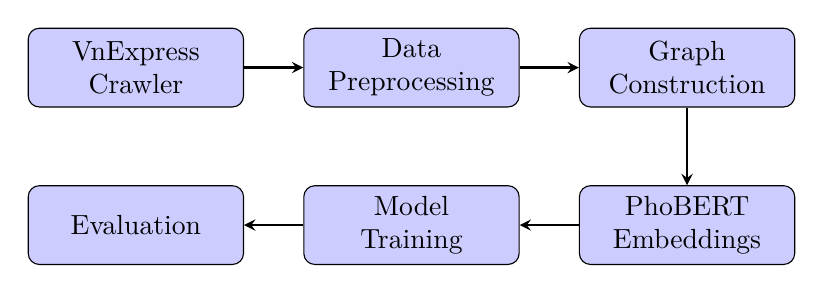
\begin{tikzpicture}[node distance=1.5cm, auto,
            block/.style={rectangle, draw, fill=blue!20, text width=2.5cm, text centered, rounded corners, minimum height=1cm},
            arrow/.style={->, >=stealth, thick}]

        \node[block] (crawl) {VnExpress\\Crawler};
        \node[block, right of=crawl, xshift=2cm] (preprocess) {Data\\Preprocessing};
        \node[block, right of=preprocess, xshift=2cm] (graph) {Graph\\Construction};
        \node[block, below of=graph, yshift=-0.5cm] (embed) {PhoBERT\\Embeddings};
        \node[block, left of=embed, xshift=-2cm] (train) {Model\\Training};
        \node[block, left of=train, xshift=-2cm] (eval) {Evaluation};

        \draw[arrow] (crawl) -- (preprocess);
        \draw[arrow] (preprocess) -- (graph);
        \draw[arrow] (graph) -- (embed);
        \draw[arrow] (embed) -- (train);
        \draw[arrow] (train) -- (eval);
    \end{tikzpicture}

    \vspace{0.5cm}
    \small
    \textbf{Pipeline:} Crawl → Clean → Build Graph → Generate Embeddings → Train → Evaluate
\end{frame}


%------------------------------------------------------------
\section{Data Collection}
%------------------------------------------------------------

\begin{frame}
    \frametitle{VnExpress Data Crawling}
    \textbf{Data Source:} VnExpress.net (largest Vietnamese news portal)

    \vspace{0.3cm}
    \textbf{Categories Crawled:}
    \begin{columns}
        \column{0.5\textwidth}
        \begin{itemize}
            \item Thời sự
            \item Thế giới
            \item Kinh doanh
            \item Giải trí
        \end{itemize}

        \column{0.5\textwidth}
        \begin{itemize}
            \item Đời sống
            \item Thể thao
            \item Khoa học
            \item Sức khỏe
        \end{itemize}
    \end{columns}

    \vspace{0.5cm}
    \textbf{Collected Data:}
    \begin{itemize}
        \item Articles: title, content, author, publish date
        \item Metadata: category, tags (per article)
        \item Comments: user ID, comment text, reactions, replies
        \item User profiles: user ID, username, join date
    \end{itemize}
\end{frame}

%------------------------------------------------------------
\section{Dataset Overview}
%------------------------------------------------------------

\begin{frame}
    \frametitle{VnExpress Dataset Statistics}
    \begin{columns}
        \column{0.5\textwidth}
        \textbf{Raw Data:}
        \begin{itemize}
            \item 3,049 Articles
            \item 13,467 Comments
            \item 12 Categories
            \item 5,636 Unique Users
        \end{itemize}

        \vspace{0.5cm}
        \textbf{Graph Data:}
        \begin{itemize}
            \item 2,991 Users
            \item 1,993 Articles
            \item 5,779 Interactions
            \item \textbf{Sparsity: 99.9\%}
        \end{itemize}

        \column{0.5\textwidth}
        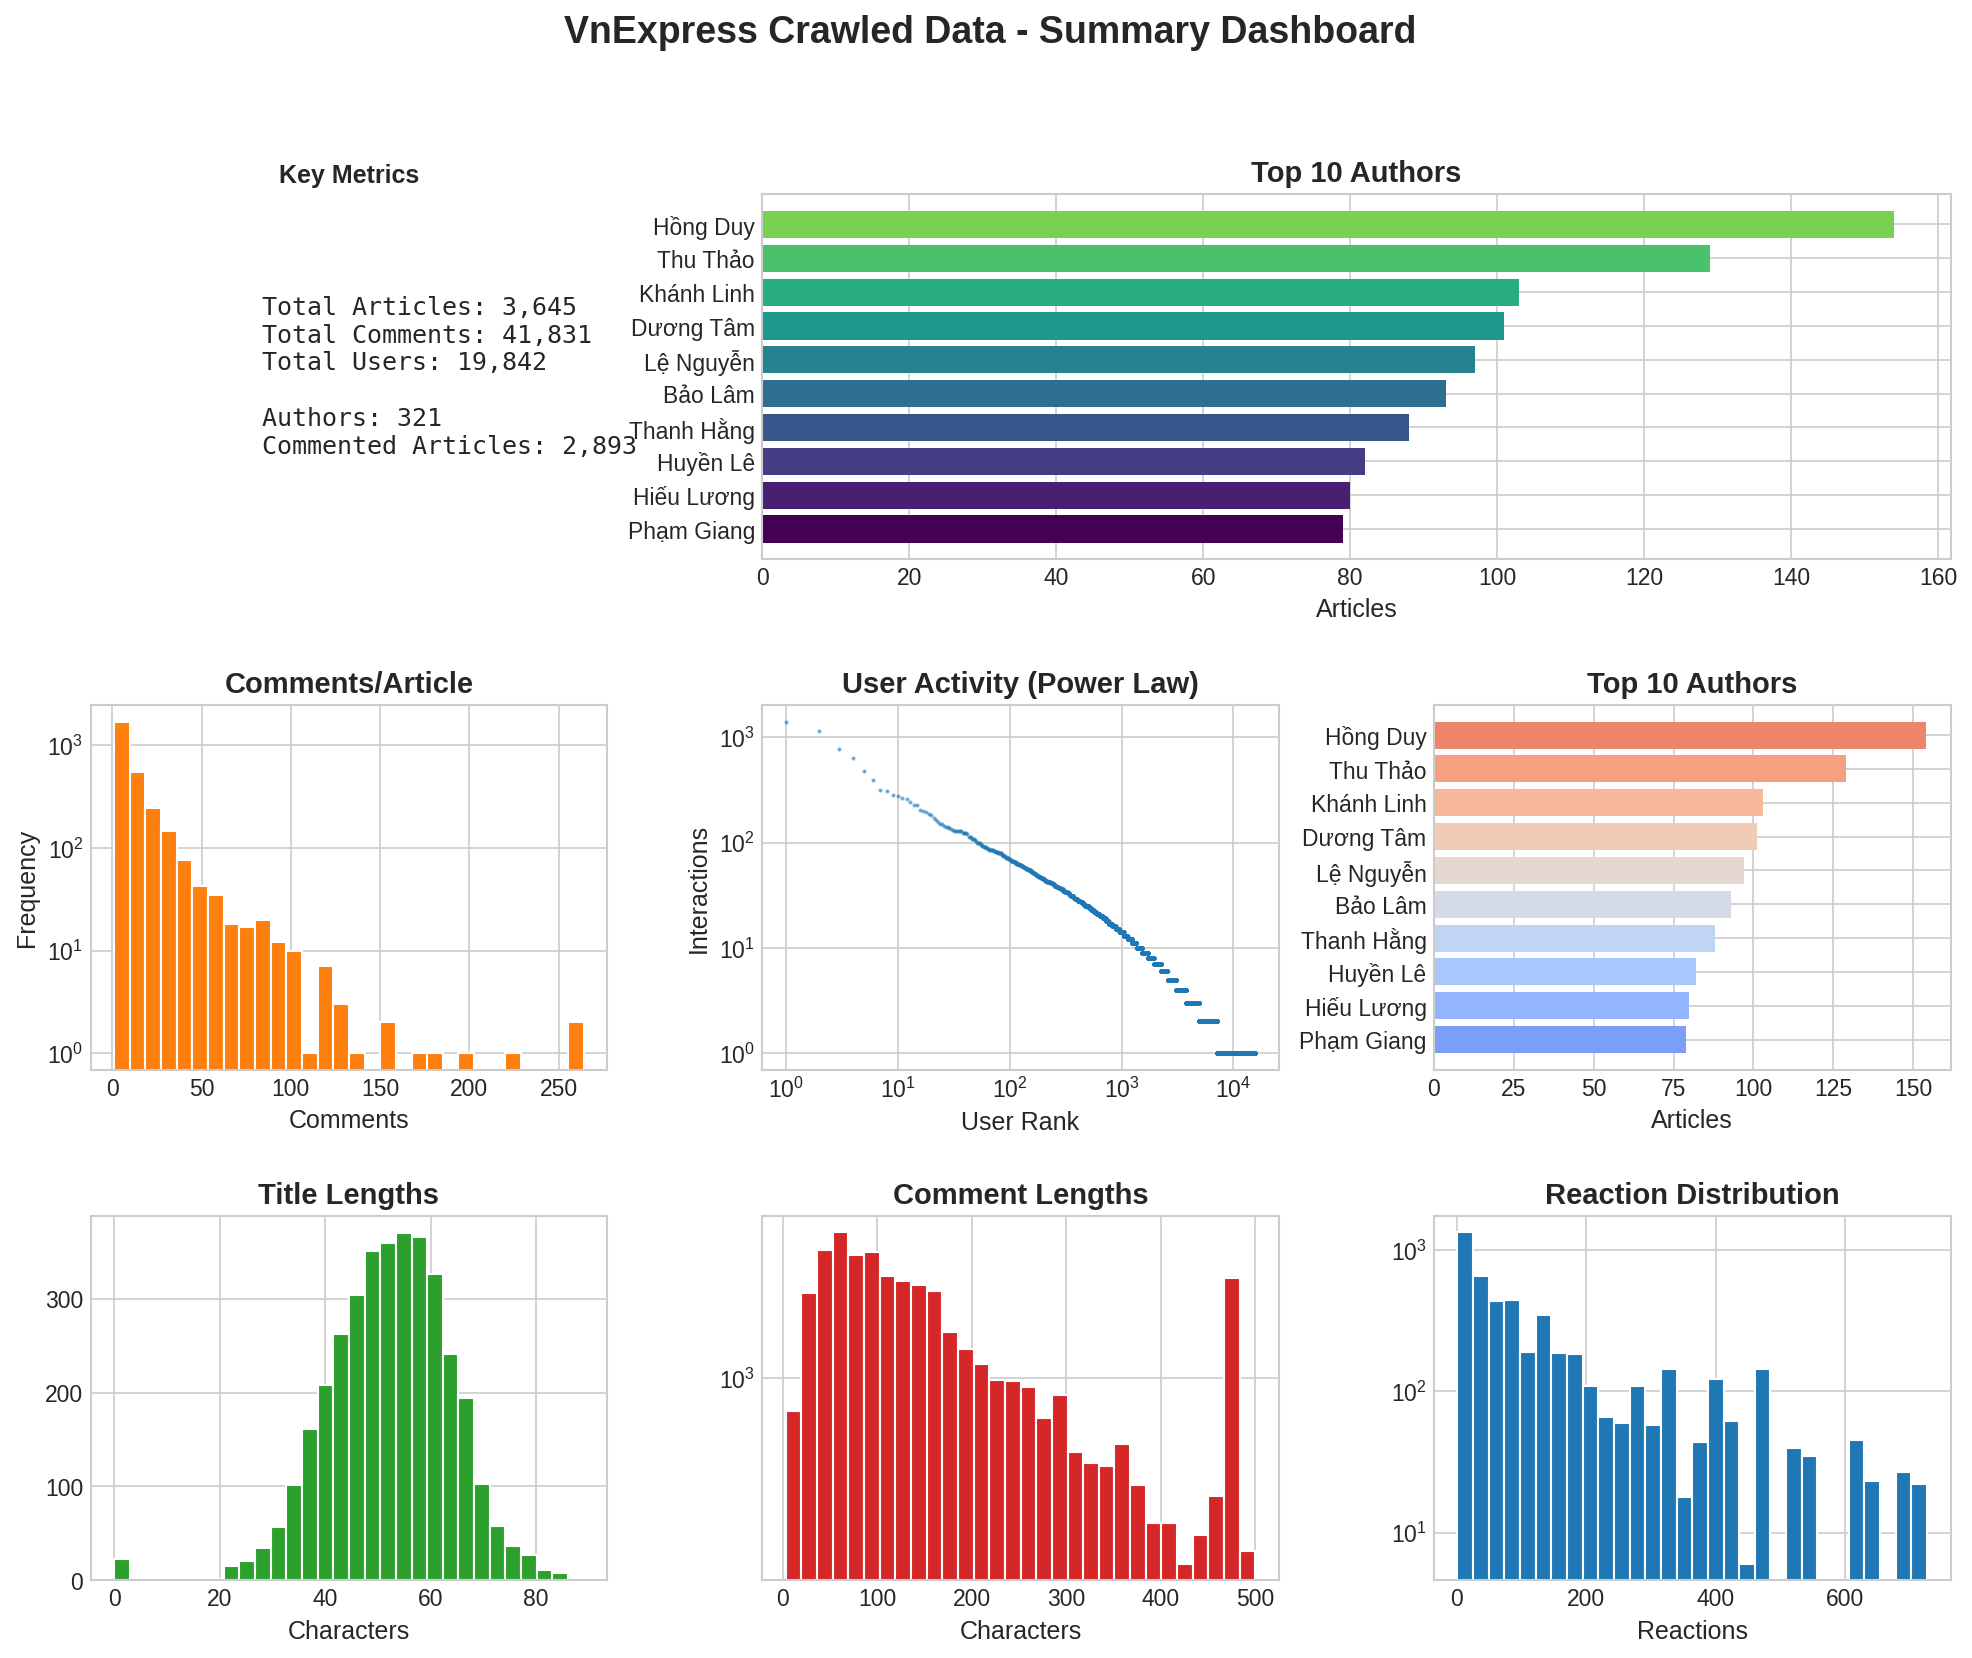
\includegraphics[width=\textwidth]{../plots/eda_00_summary_dashboard.png}
    \end{columns}
\end{frame}

% %------------------------------------------------------------
% \section{Exploratory Data Analysis}
% %------------------------------------------------------------

% \begin{frame}
%     \frametitle{Category Distribution}
%     \centering
%     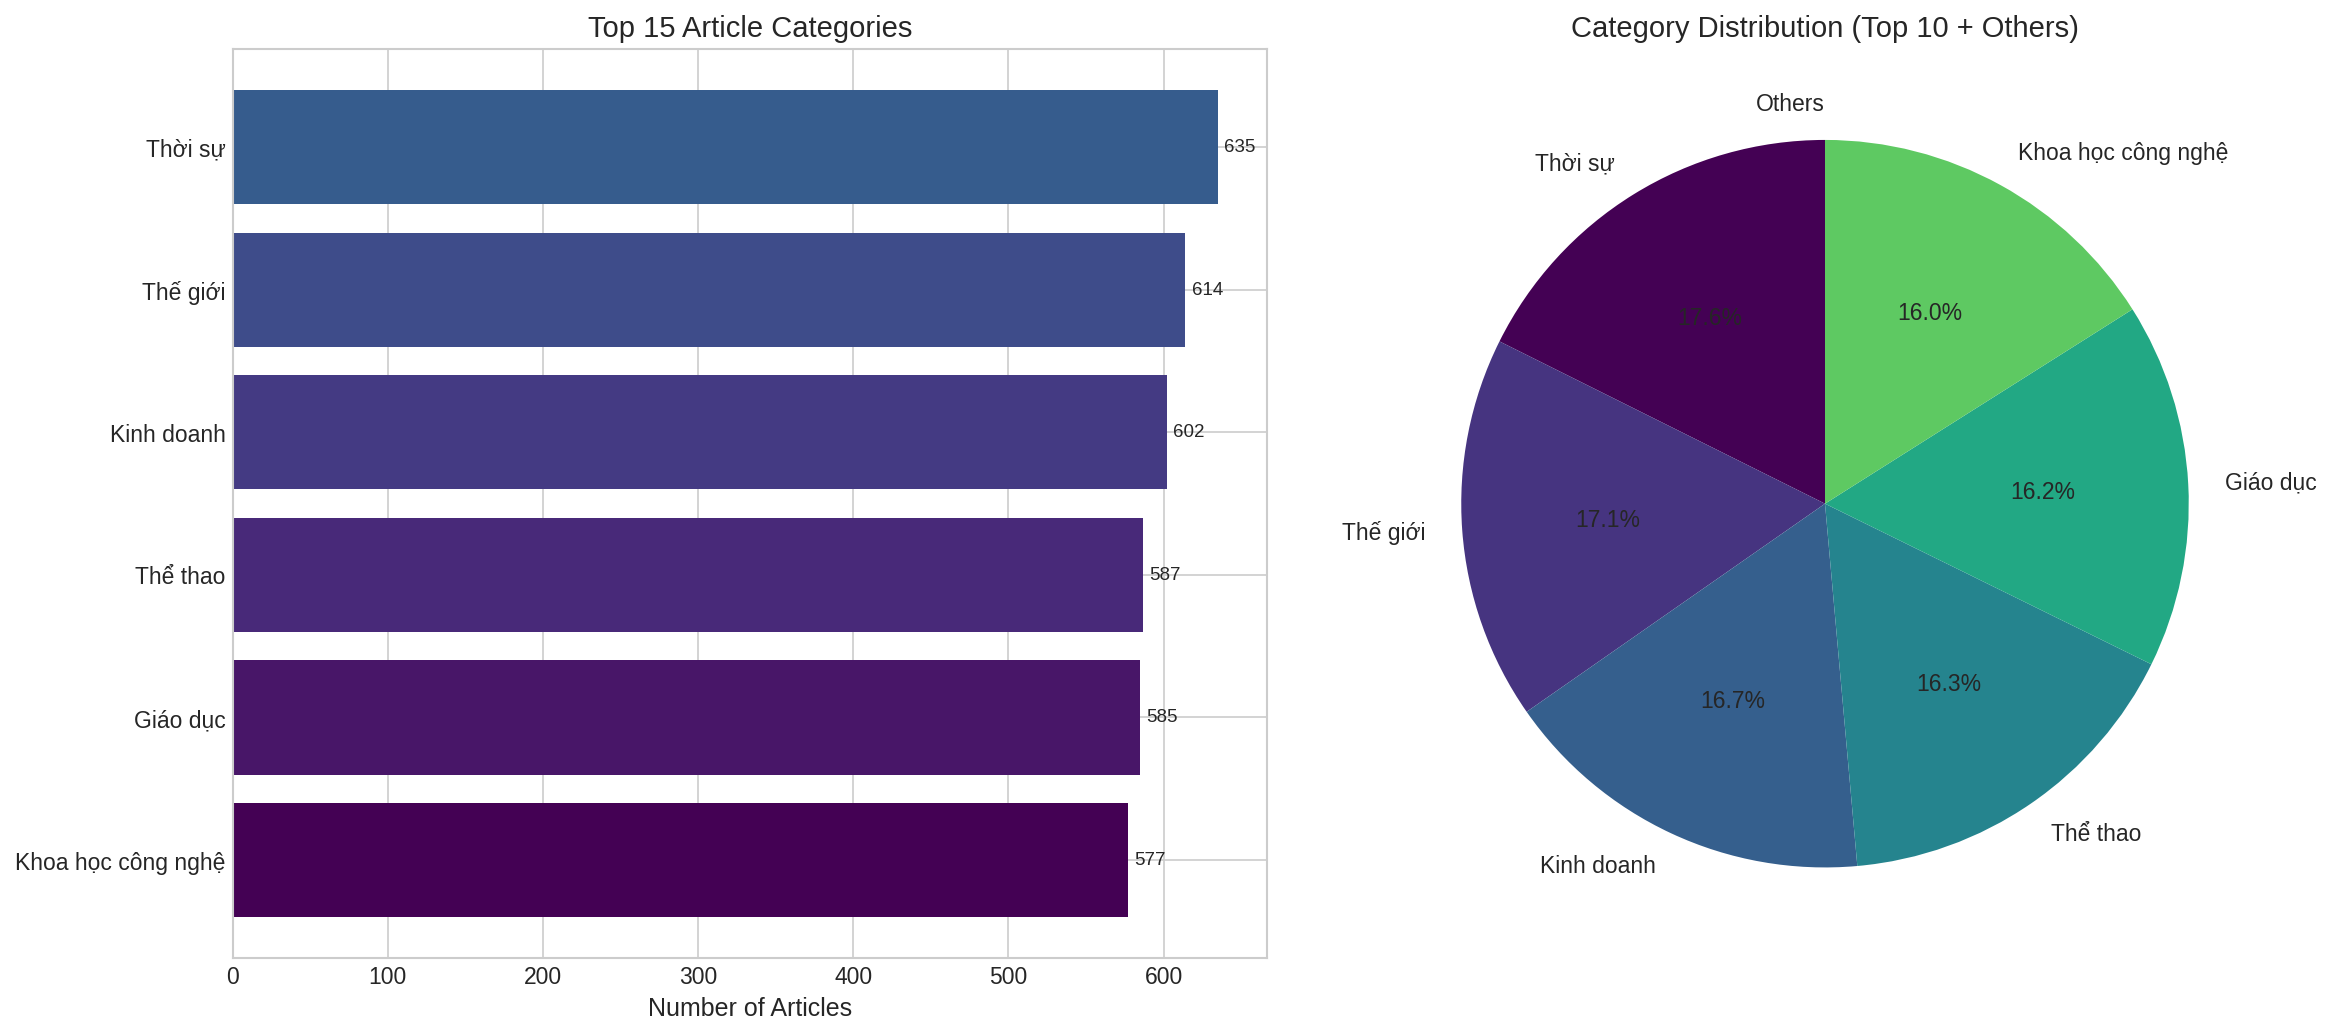
\includegraphics[width=0.9\textwidth]{../plots/eda_09_metadata_categories.png}
% \end{frame}

% \begin{frame}
%     \frametitle{Tags Distribution}
%     \centering
%     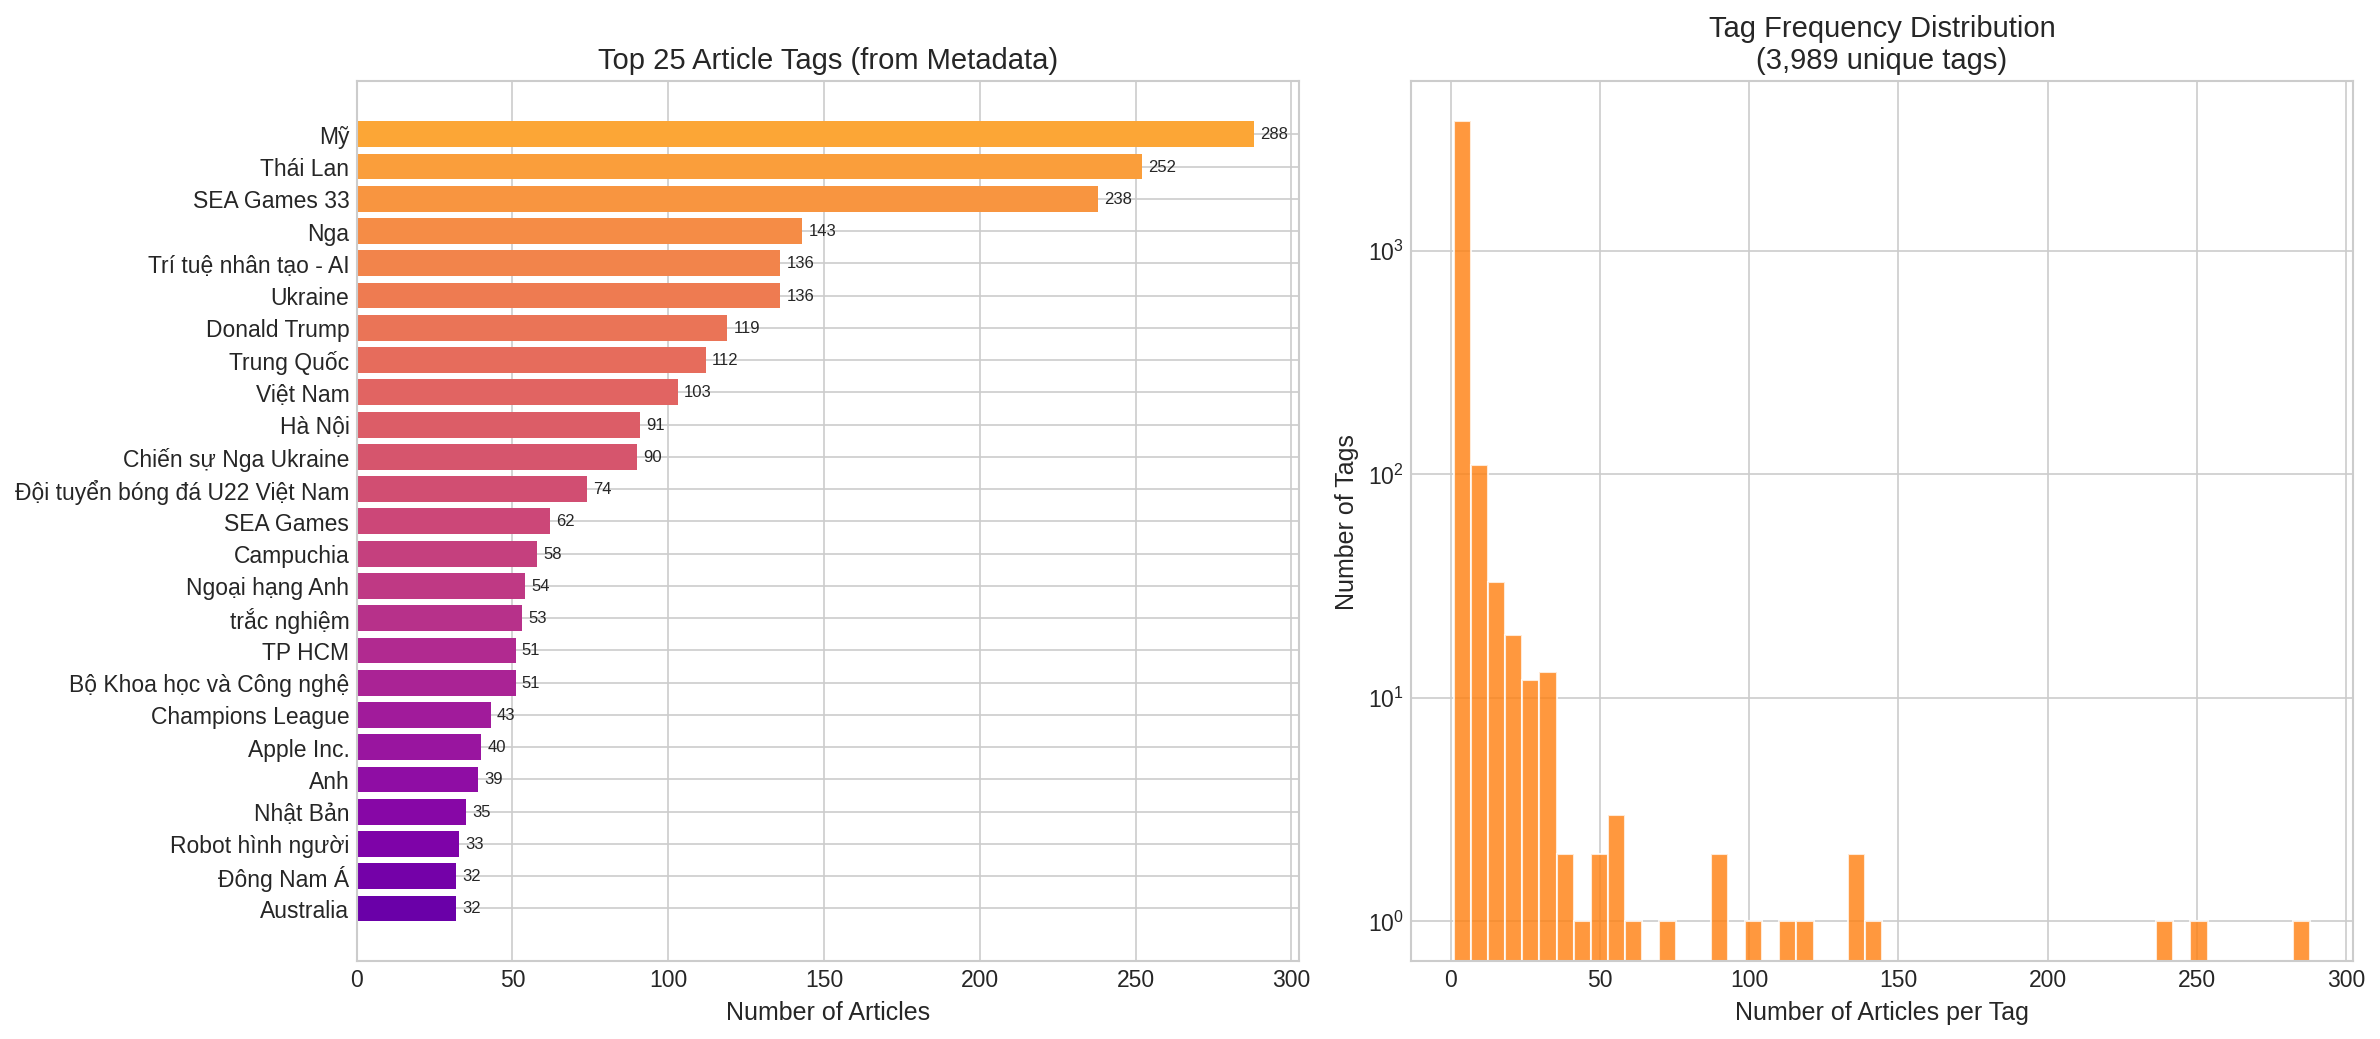
\includegraphics[width=0.9\textwidth]{../plots/eda_10_metadata_tags.png}
% \end{frame}

% \begin{frame}
%     \frametitle{Comments per Article}
%     \centering
%     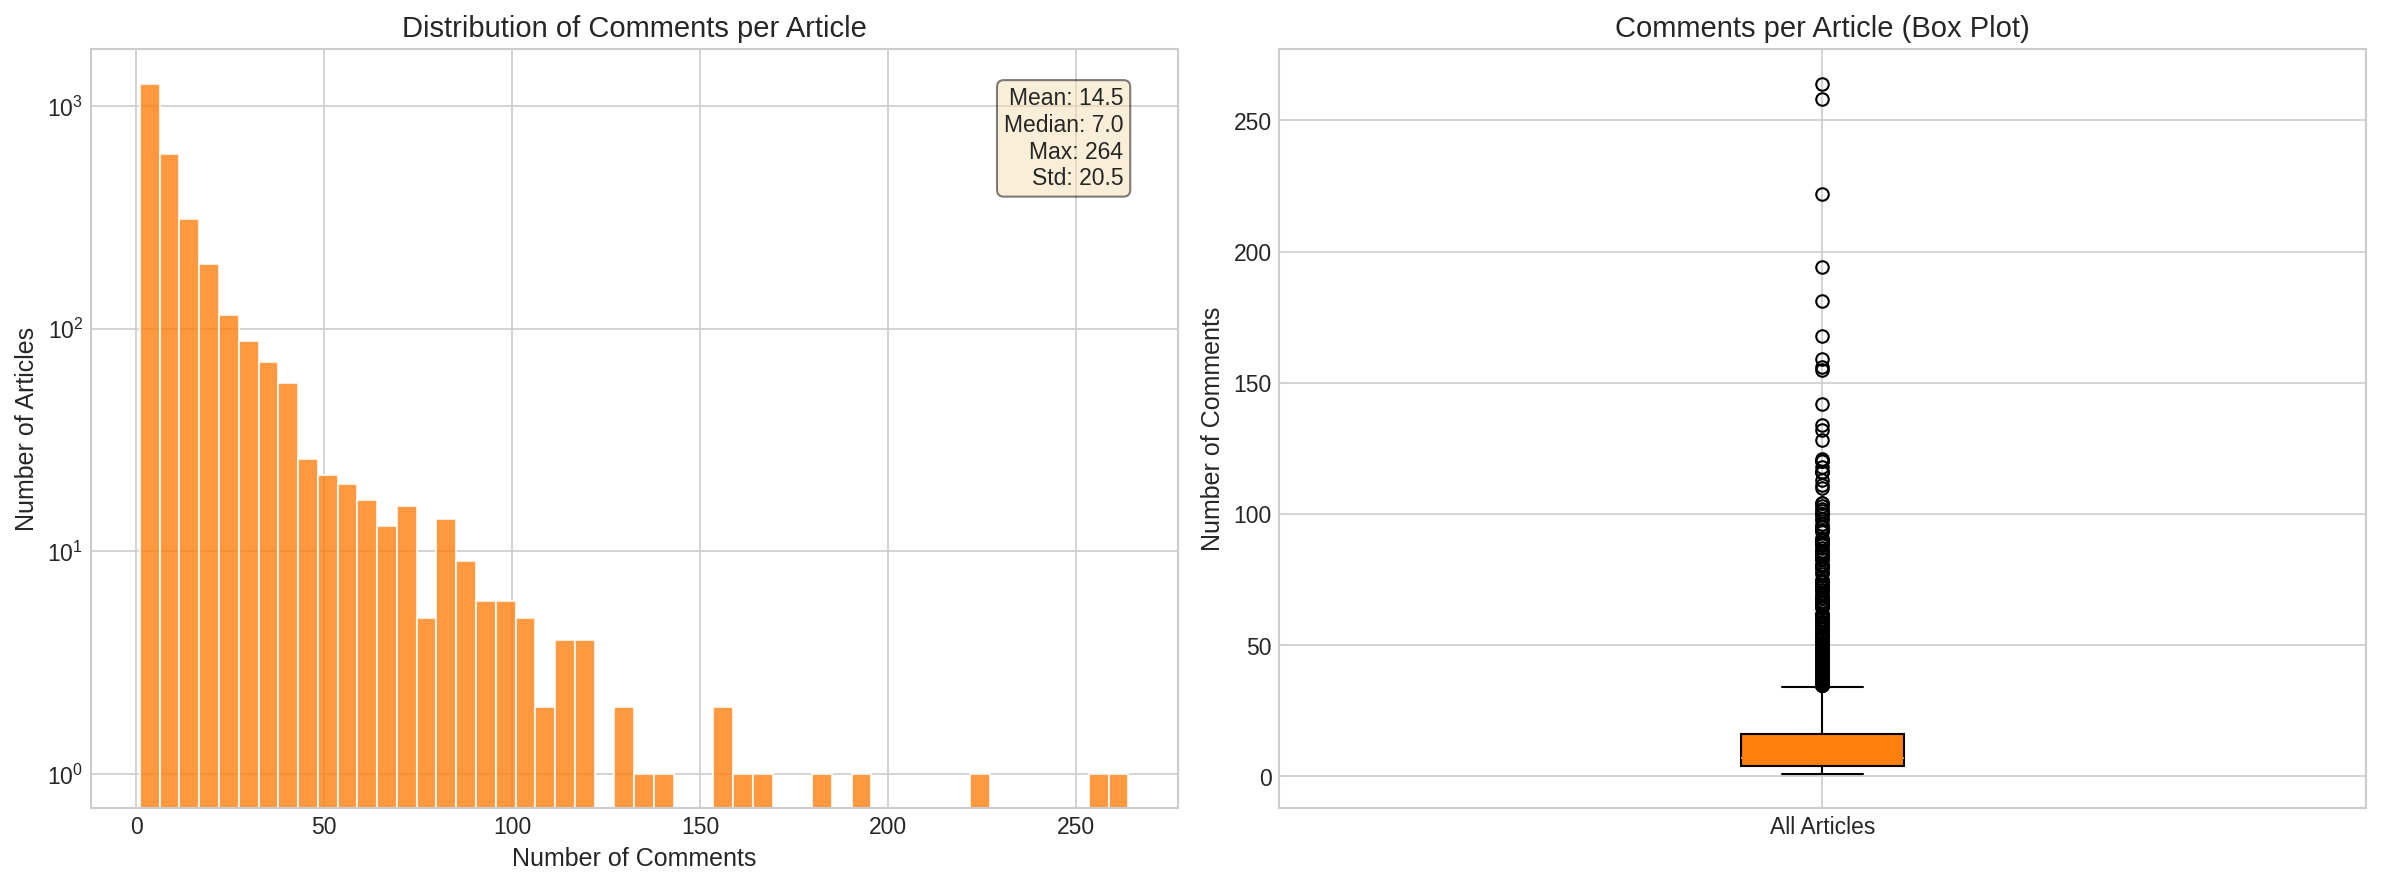
\includegraphics[width=0.9\textwidth]{../plots/eda_02_comments_per_article.png}
% \end{frame}

% \begin{frame}
%     \frametitle{User Activity Patterns (Power Law)}
%     \centering
%     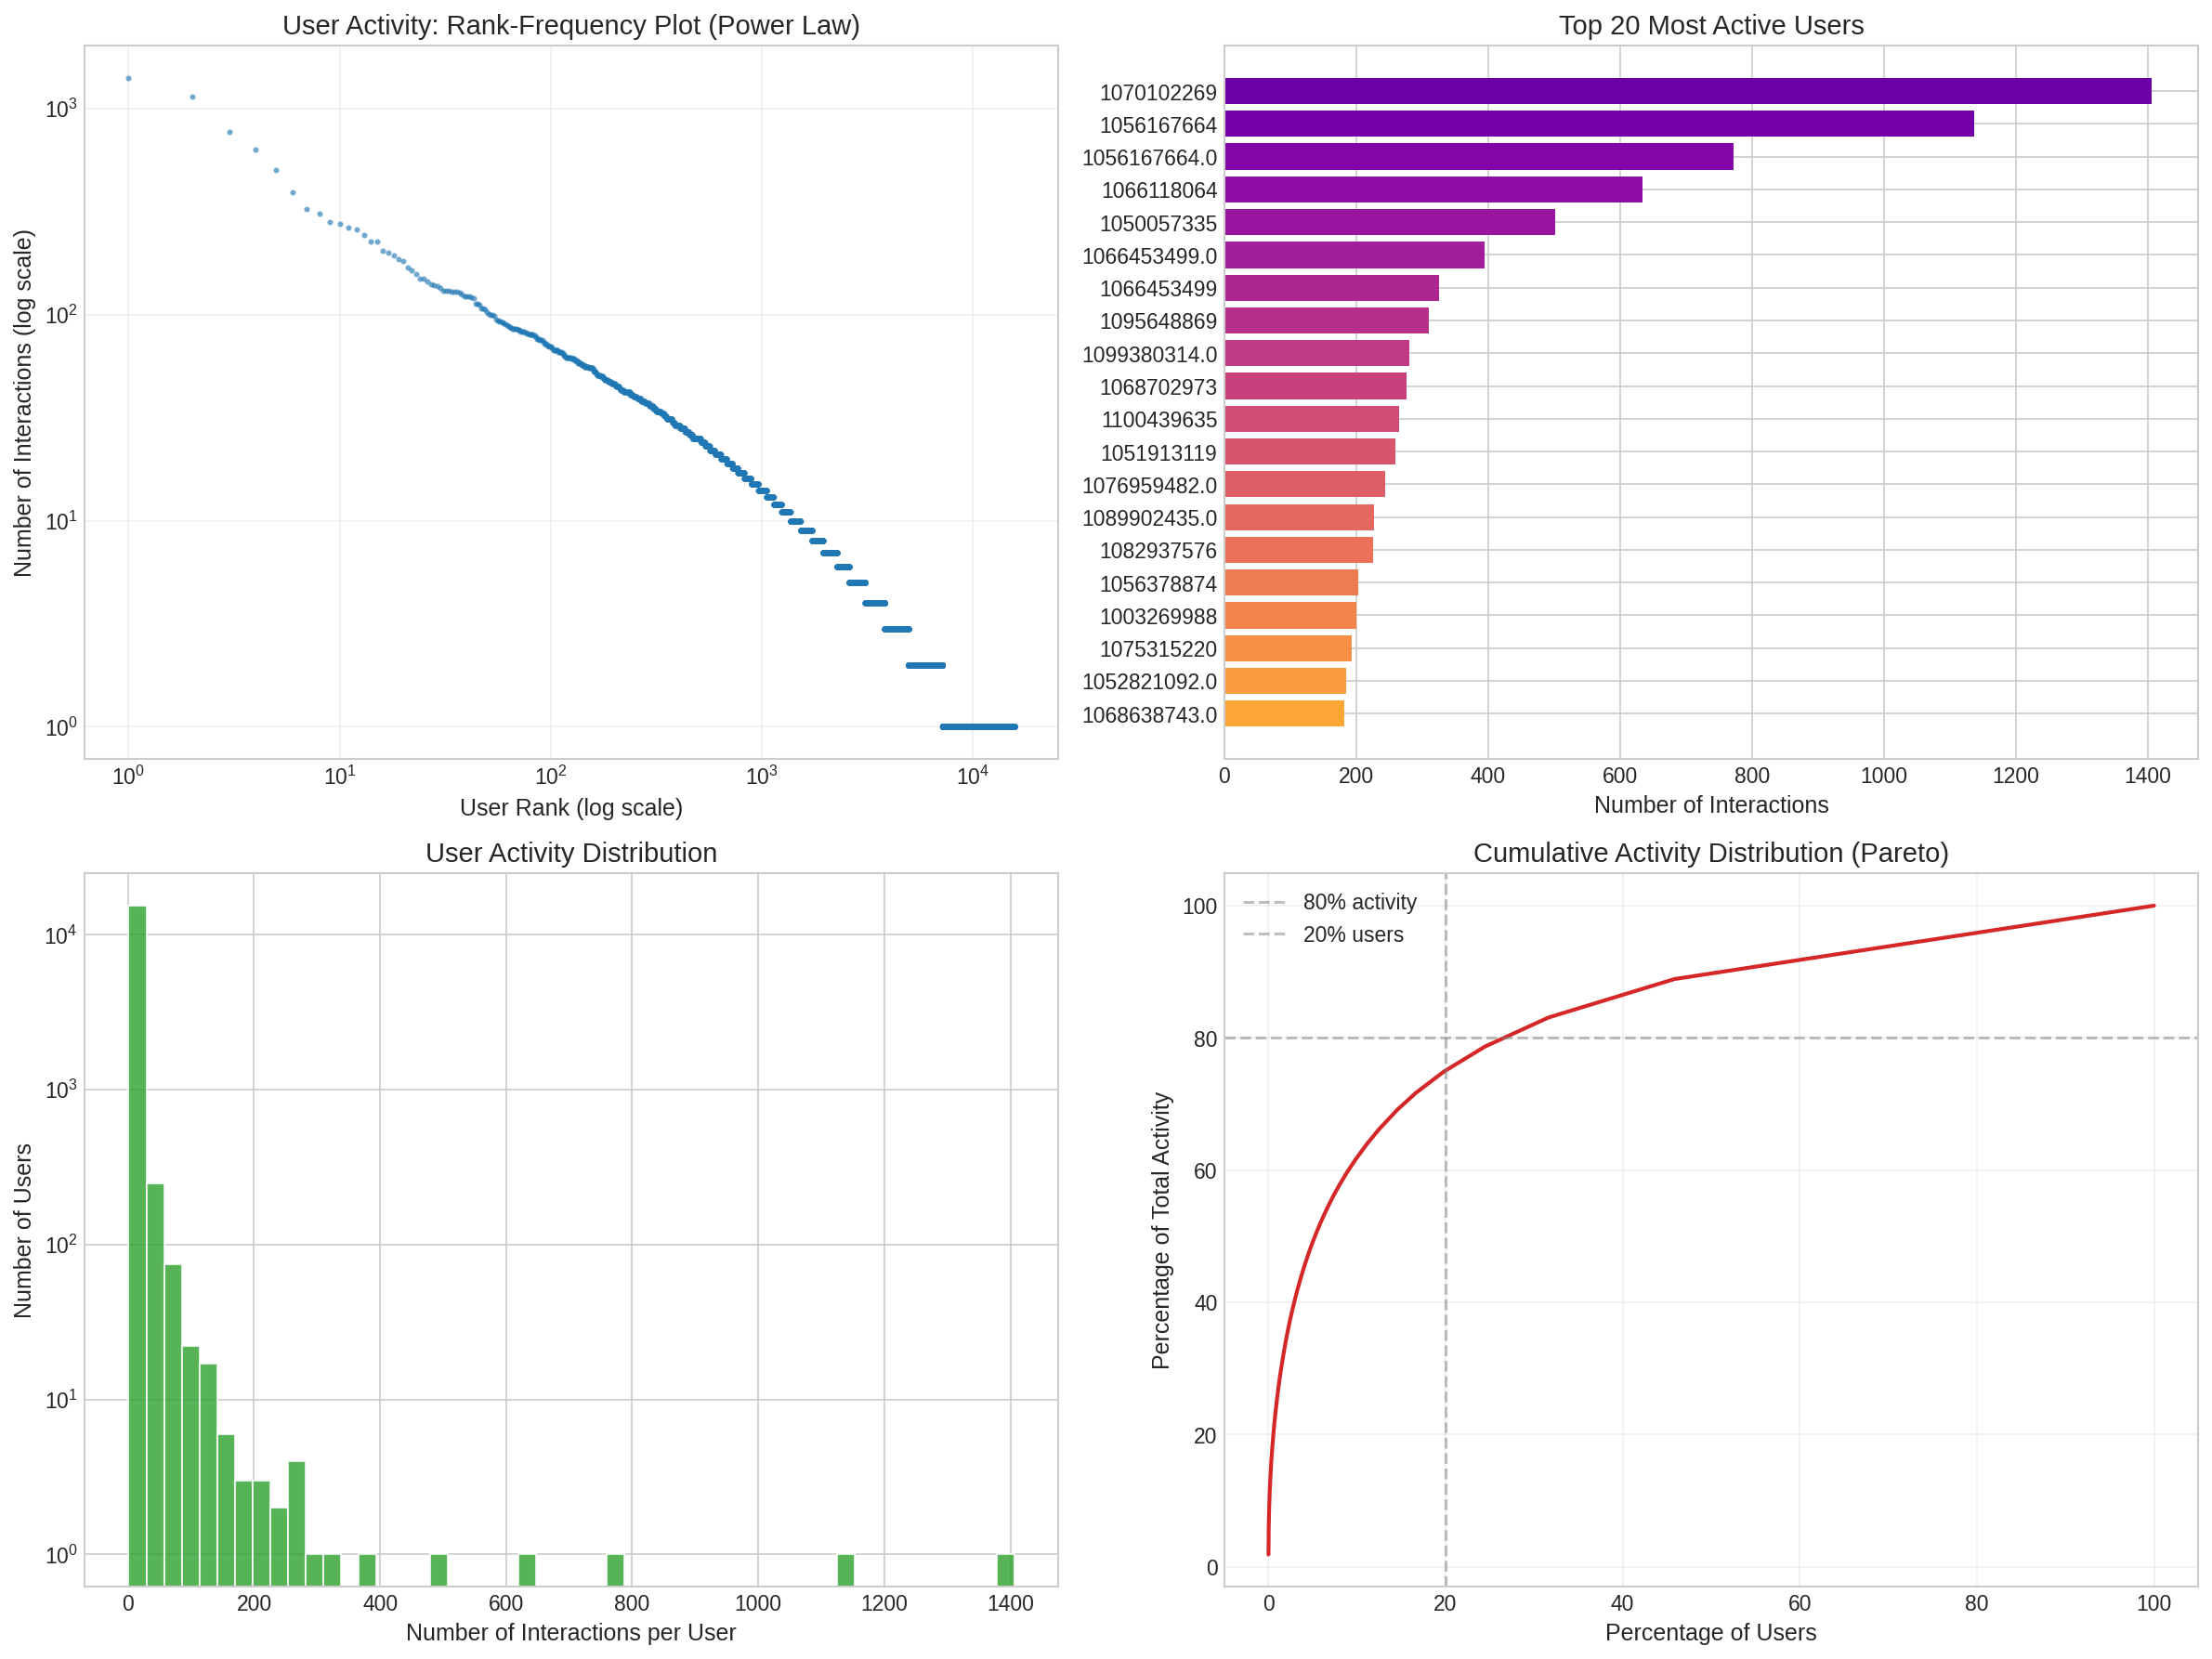
\includegraphics[width=0.85\textwidth]{../plots/eda_03_user_activity.png}
% \end{frame}

% \begin{frame}
%     \frametitle{Reaction Patterns}
%     \centering
%     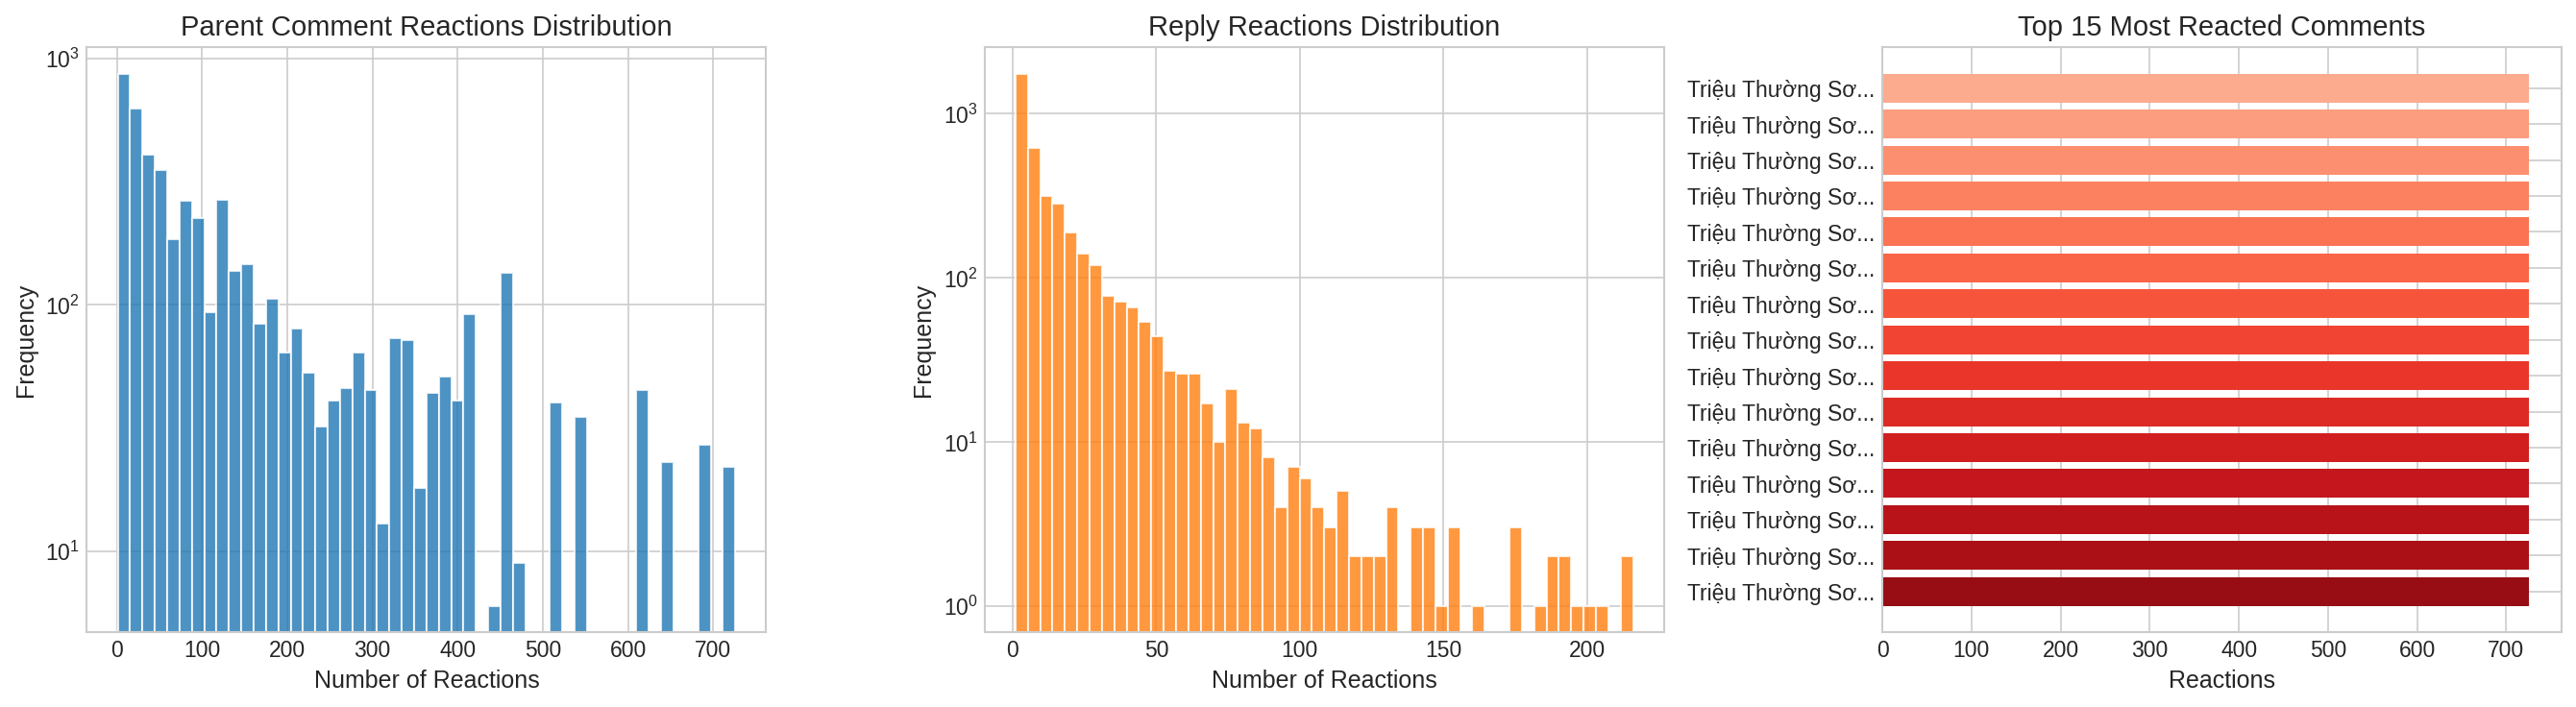
\includegraphics[width=0.9\textwidth]{../plots/eda_04_reactions.png}
% \end{frame}

% \begin{frame}
%     \frametitle{Text Length Distributions}
%     \centering
%     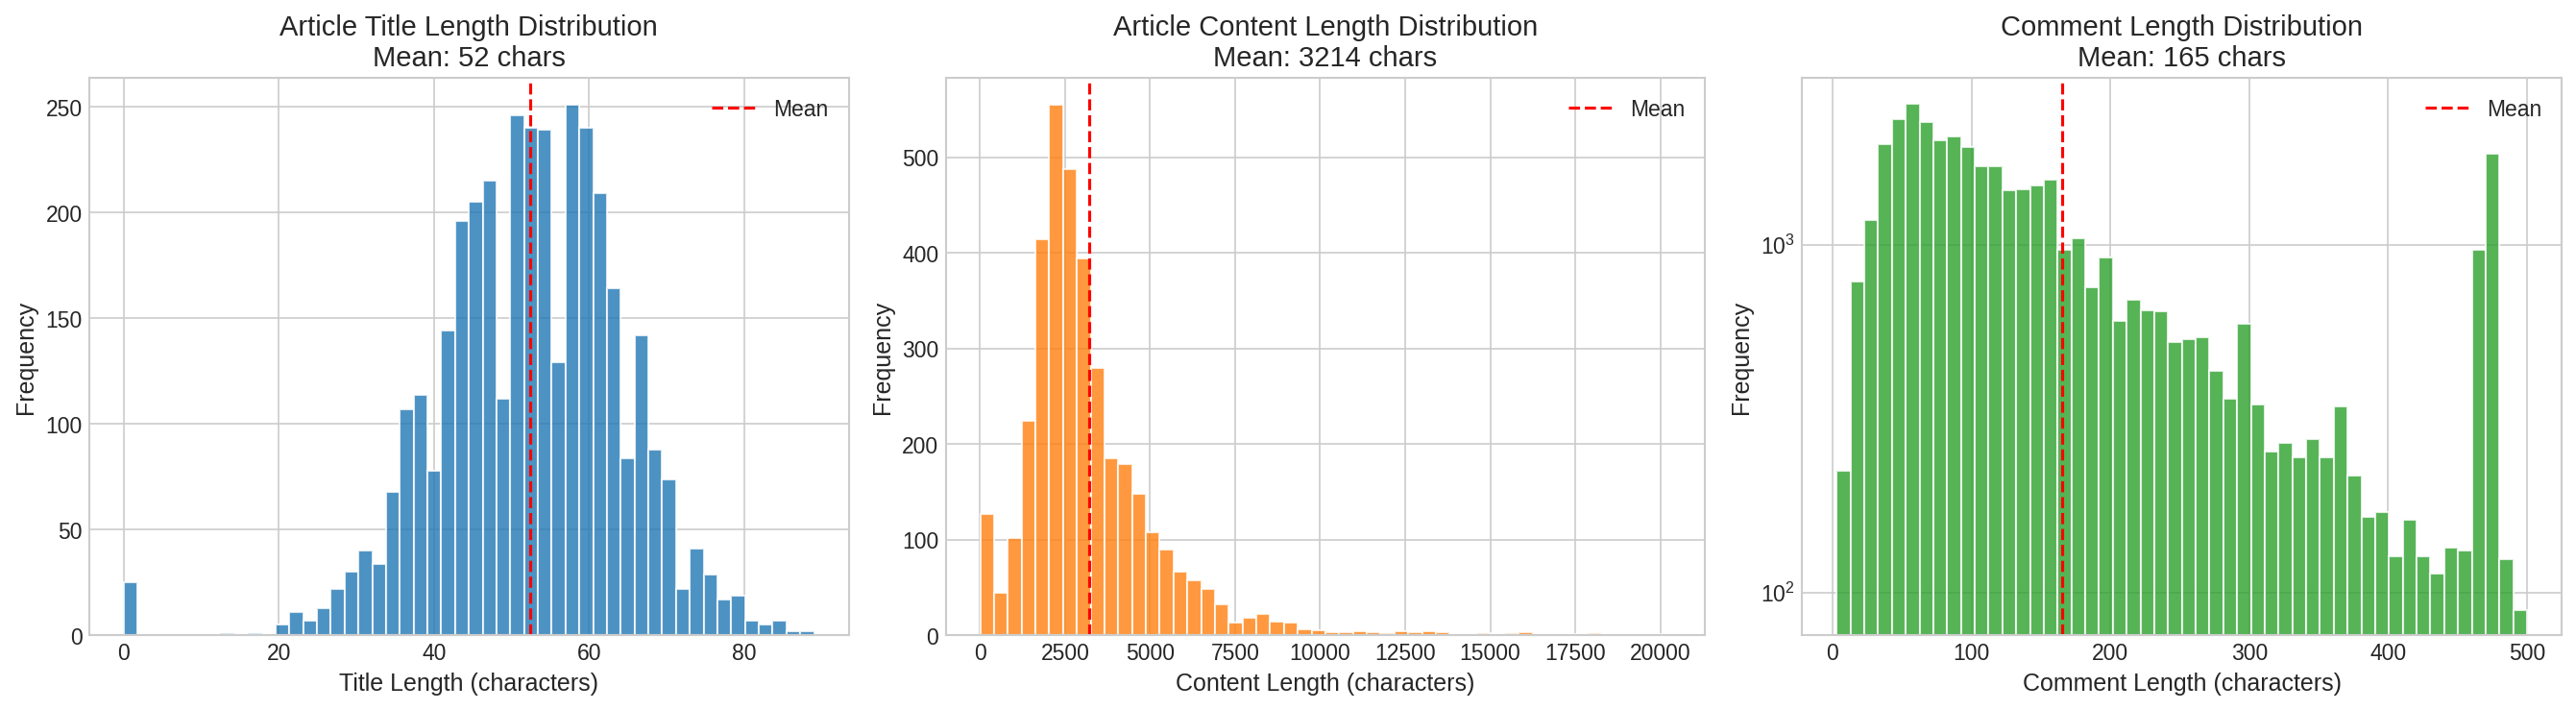
\includegraphics[width=0.9\textwidth]{../plots/eda_05_text_lengths.png}
% \end{frame}

% \begin{frame}
%     \frametitle{Reply Patterns}
%     \centering
%     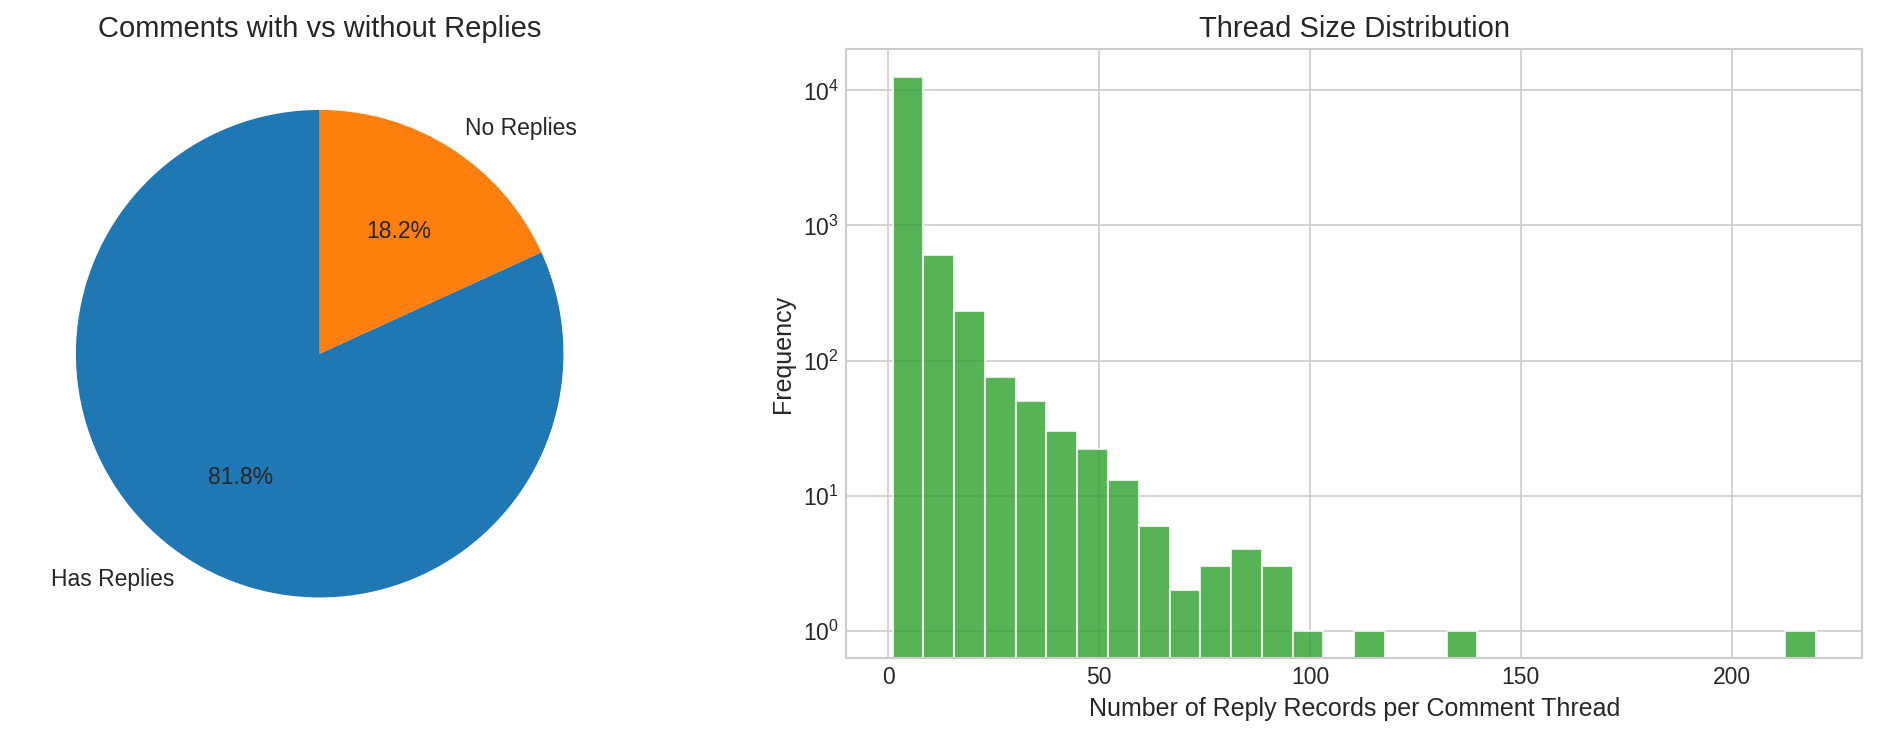
\includegraphics[width=0.9\textwidth]{../plots/eda_06_reply_patterns.png}
% \end{frame}

% \begin{frame}
%     \frametitle{Author Productivity}
%     \centering
%     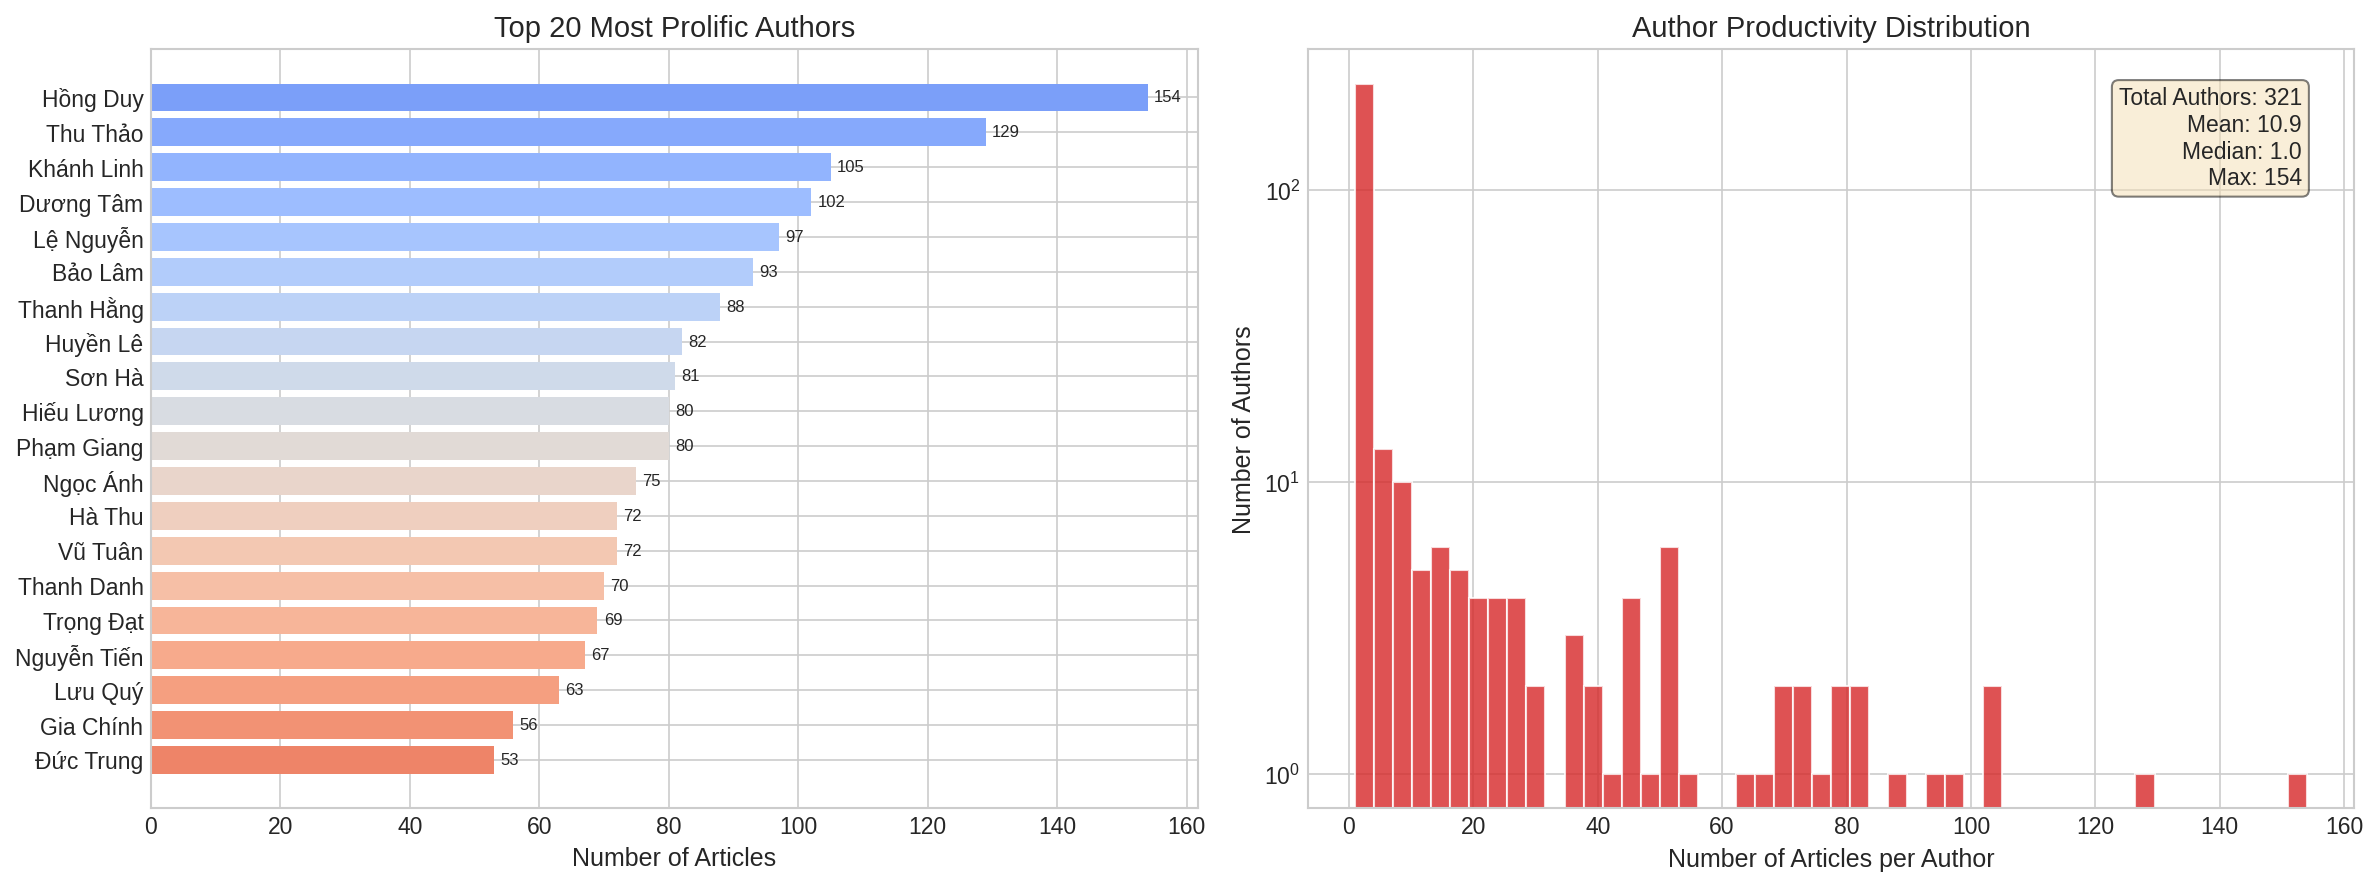
\includegraphics[width=0.9\textwidth]{../plots/eda_07_author_productivity.png}
% \end{frame}

% \begin{frame}
%     \frametitle{Top Engaged Articles}
%     \centering
%     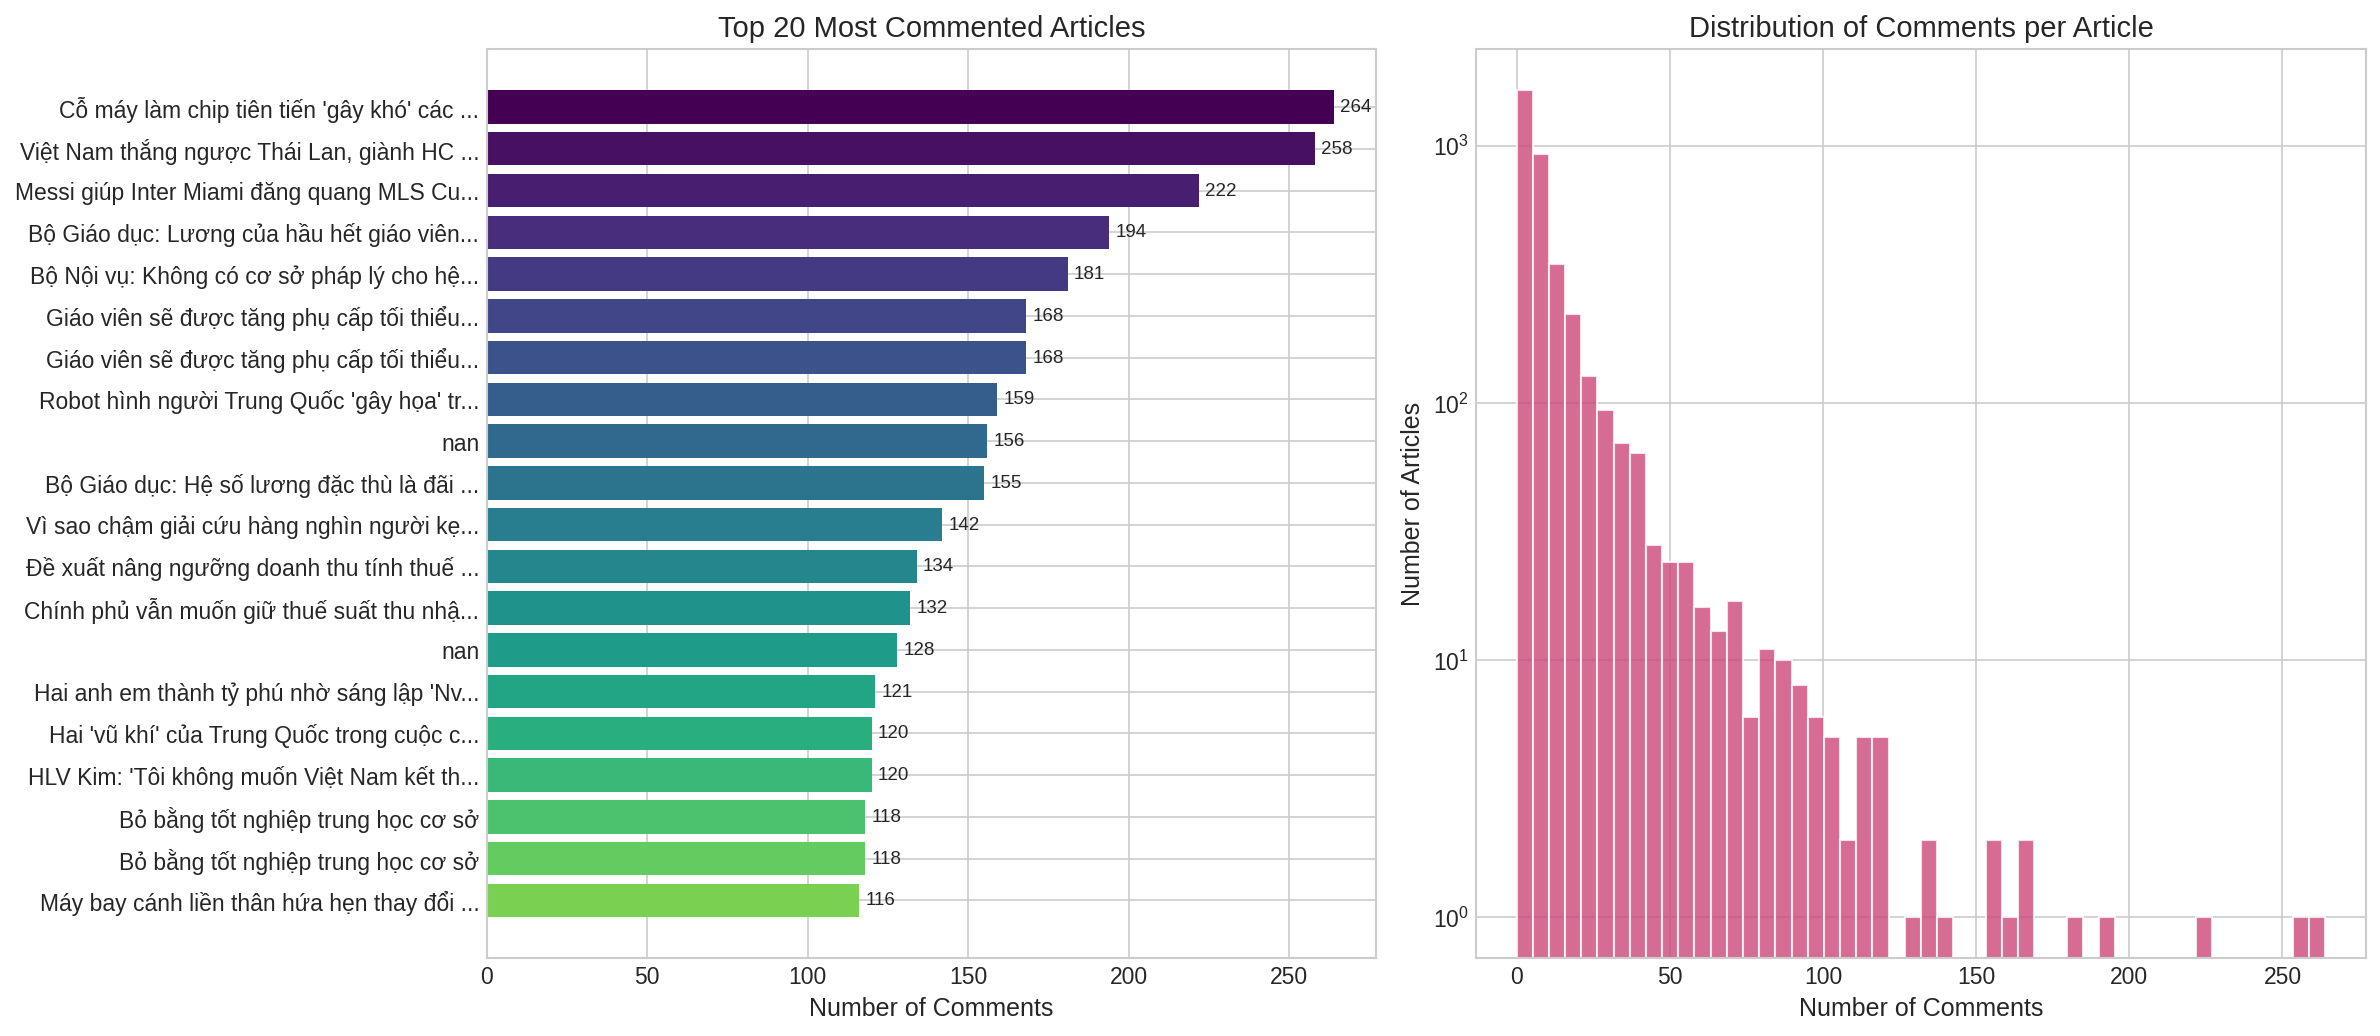
\includegraphics[width=0.9\textwidth]{../plots/eda_08_engagement_patterns.png}
% \end{frame}

% \begin{frame}
%     \frametitle{Engagement by Category}
%     \centering
%     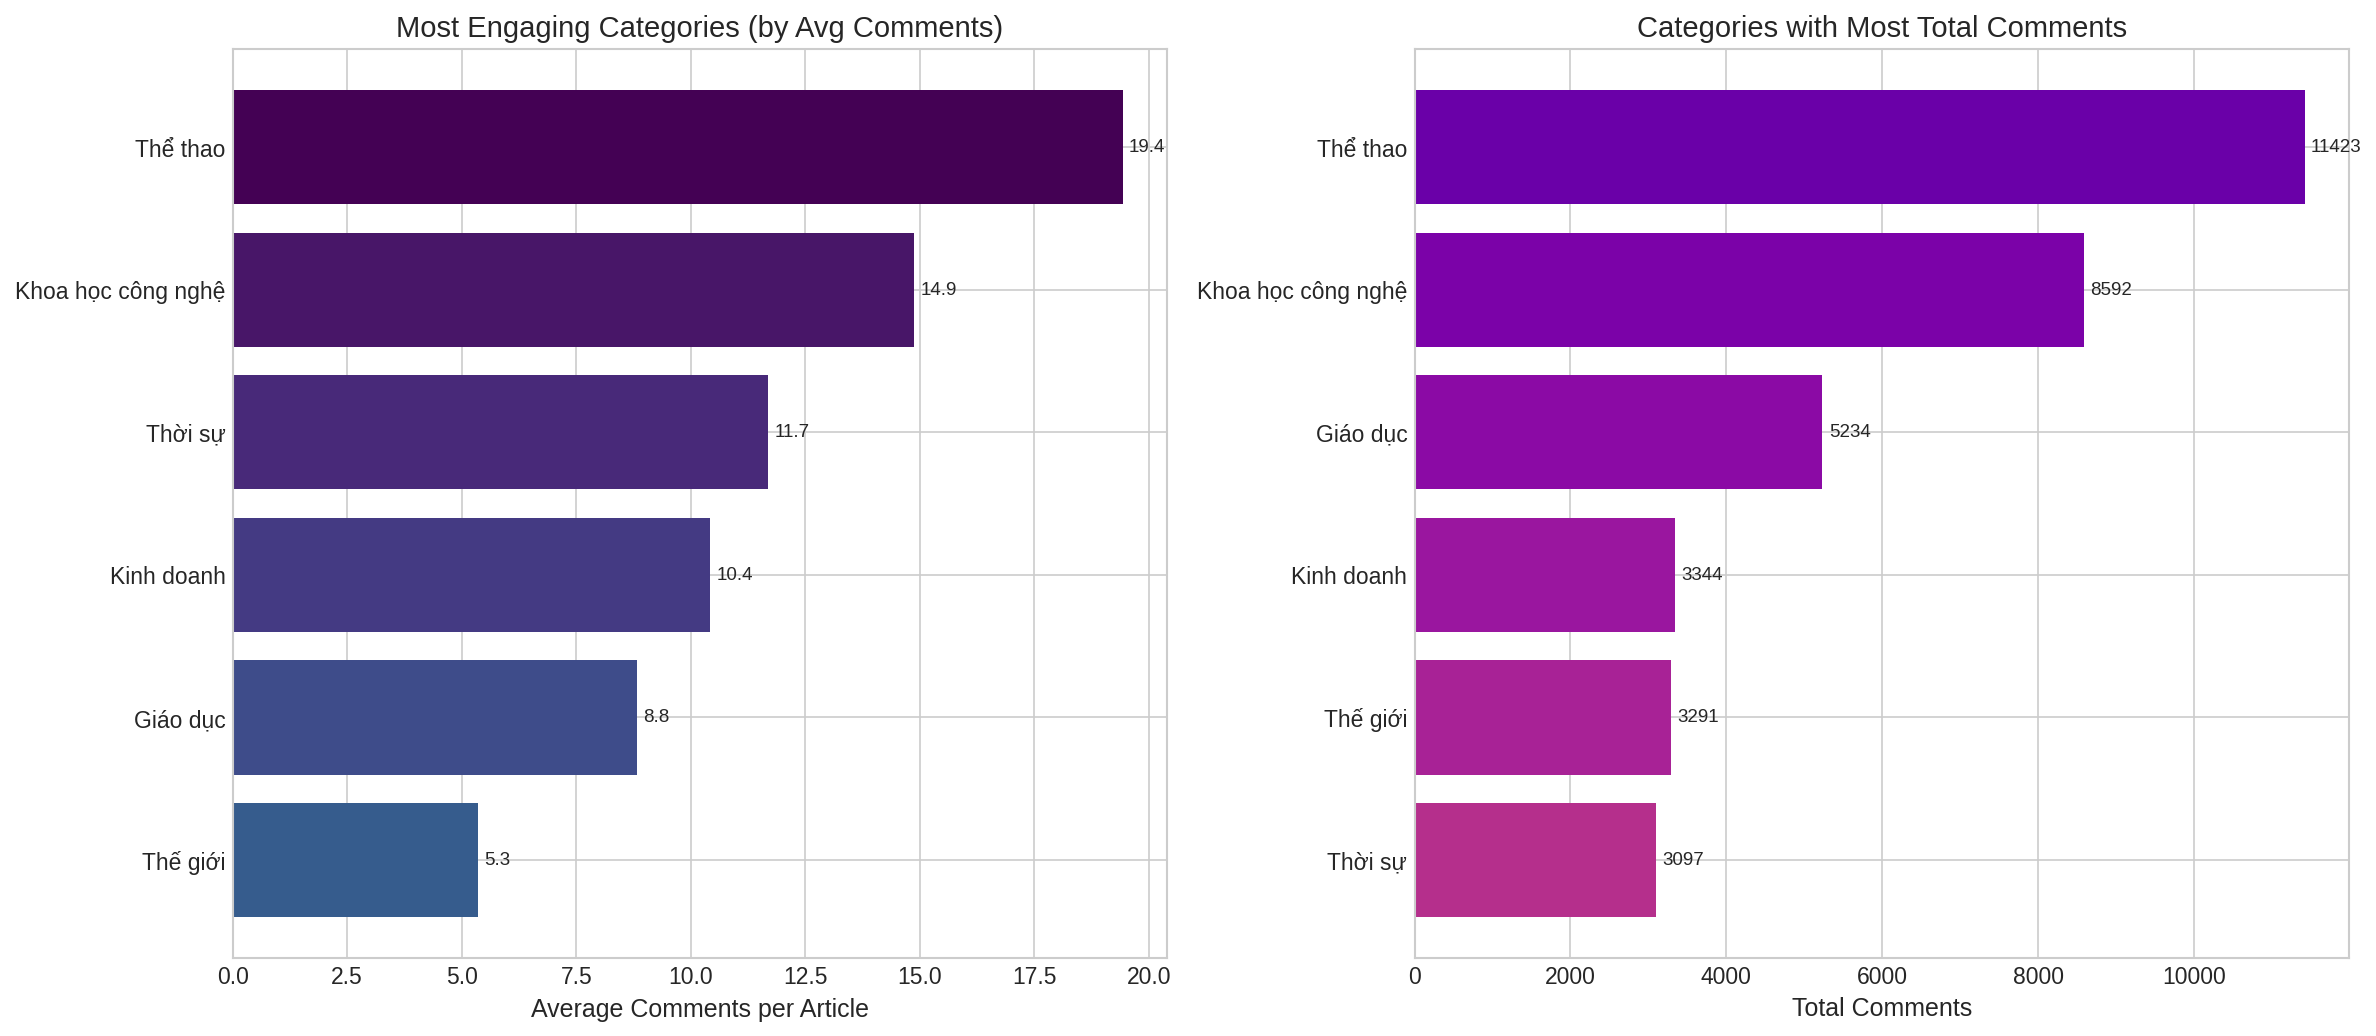
\includegraphics[width=0.9\textwidth]{../plots/eda_11_engagement_by_category.png}
% \end{frame}

% %------------------------------------------------------------
% \section{Graph Analysis}
% %------------------------------------------------------------

% \begin{frame}
%     \frametitle{Graph Summary}
%     \centering
%     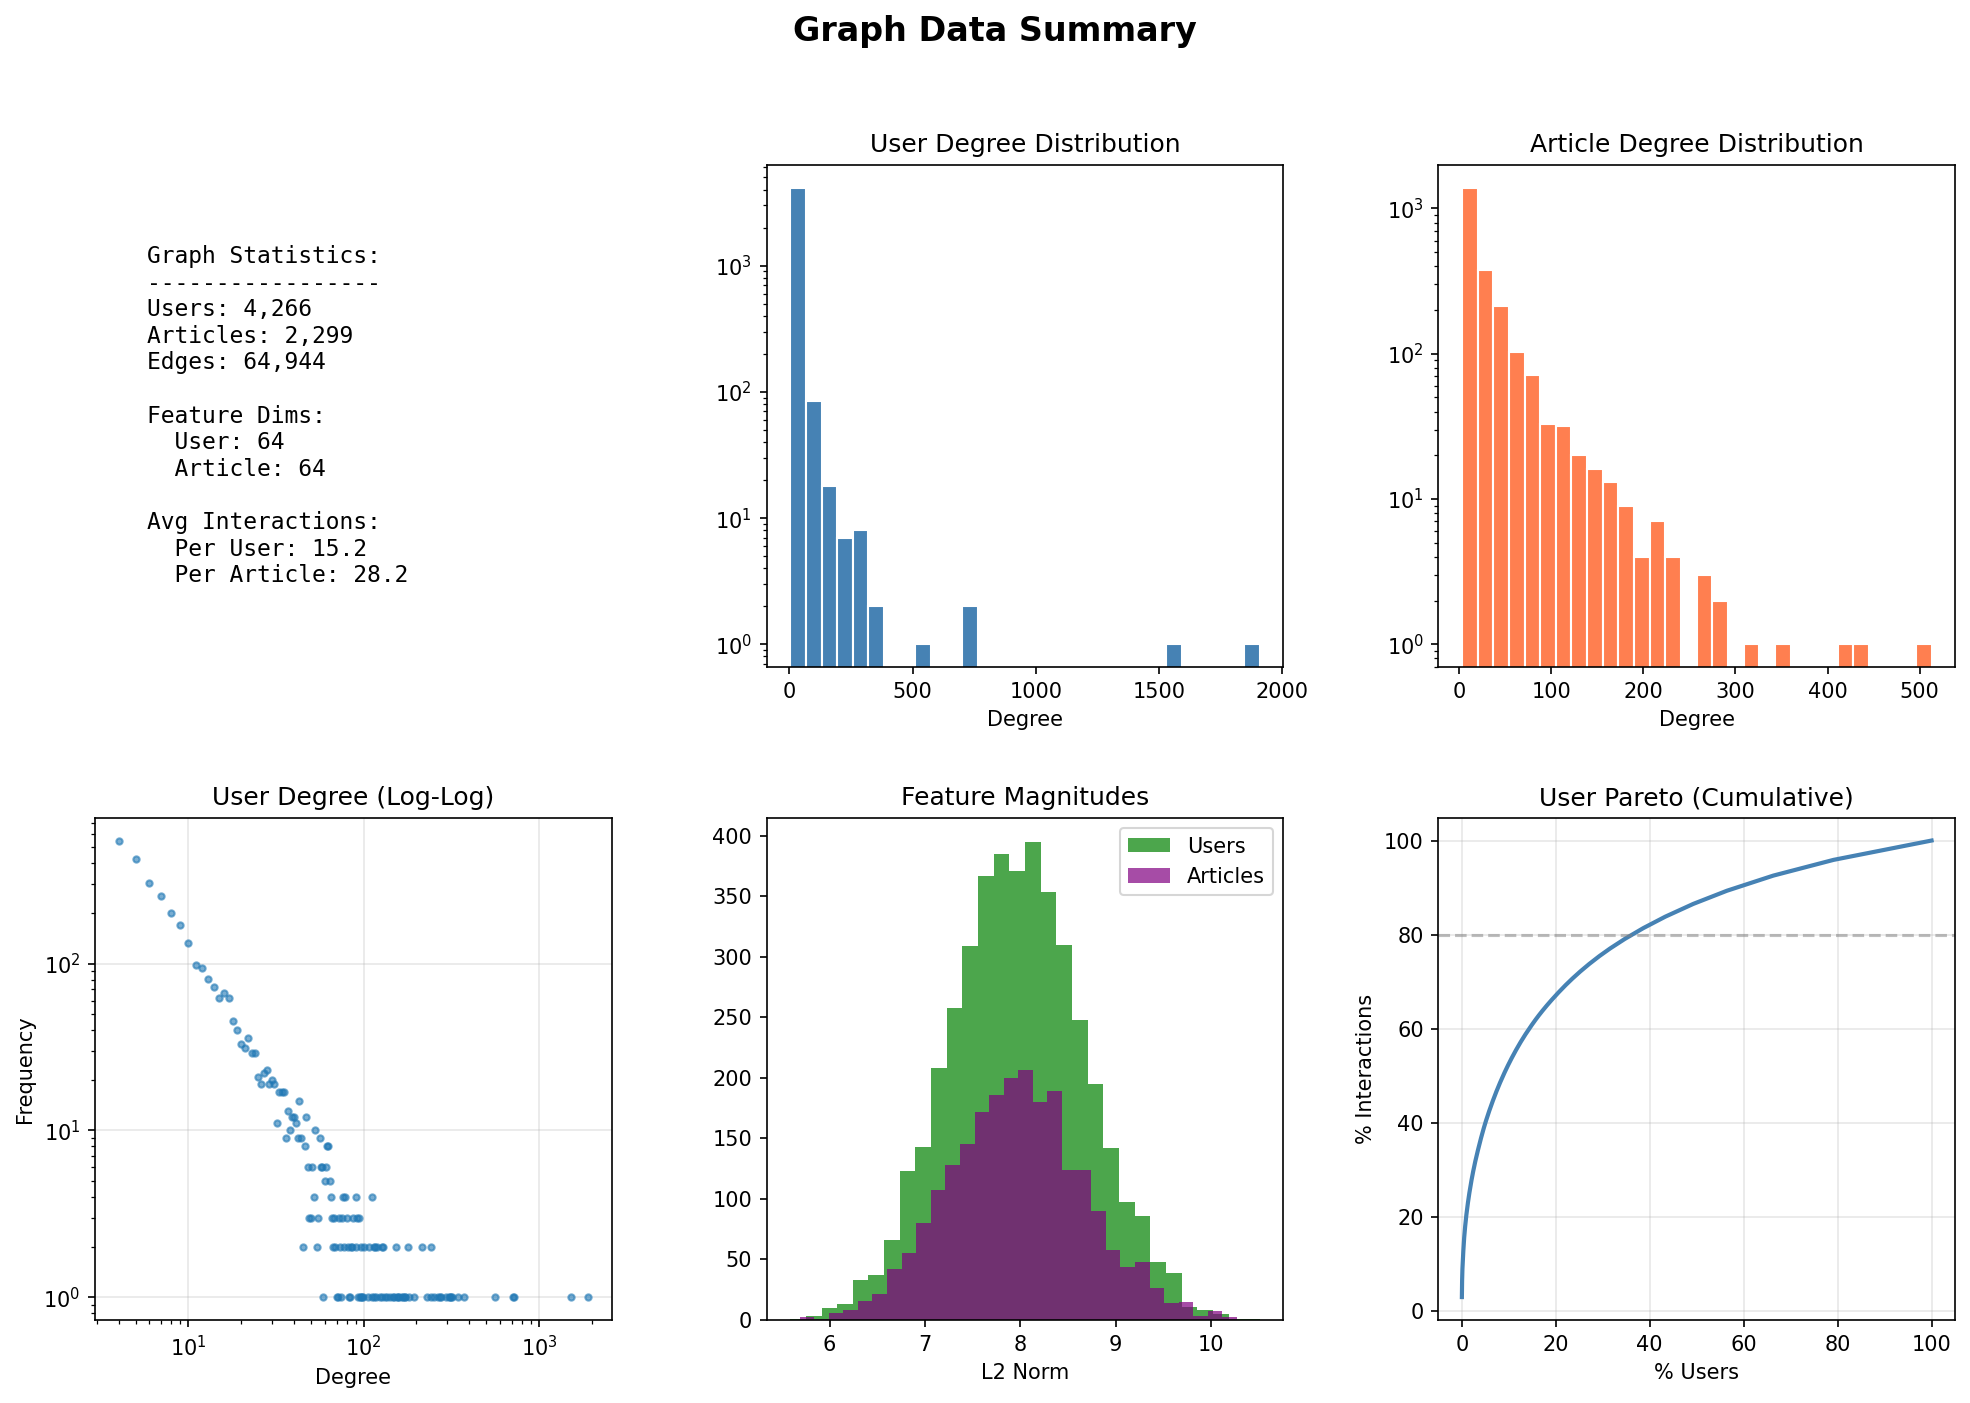
\includegraphics[width=0.85\textwidth]{../plots/graph_eda_00_summary.png}
% \end{frame}

% \begin{frame}
%     \frametitle{Node Degree Distribution}
%     \centering
%     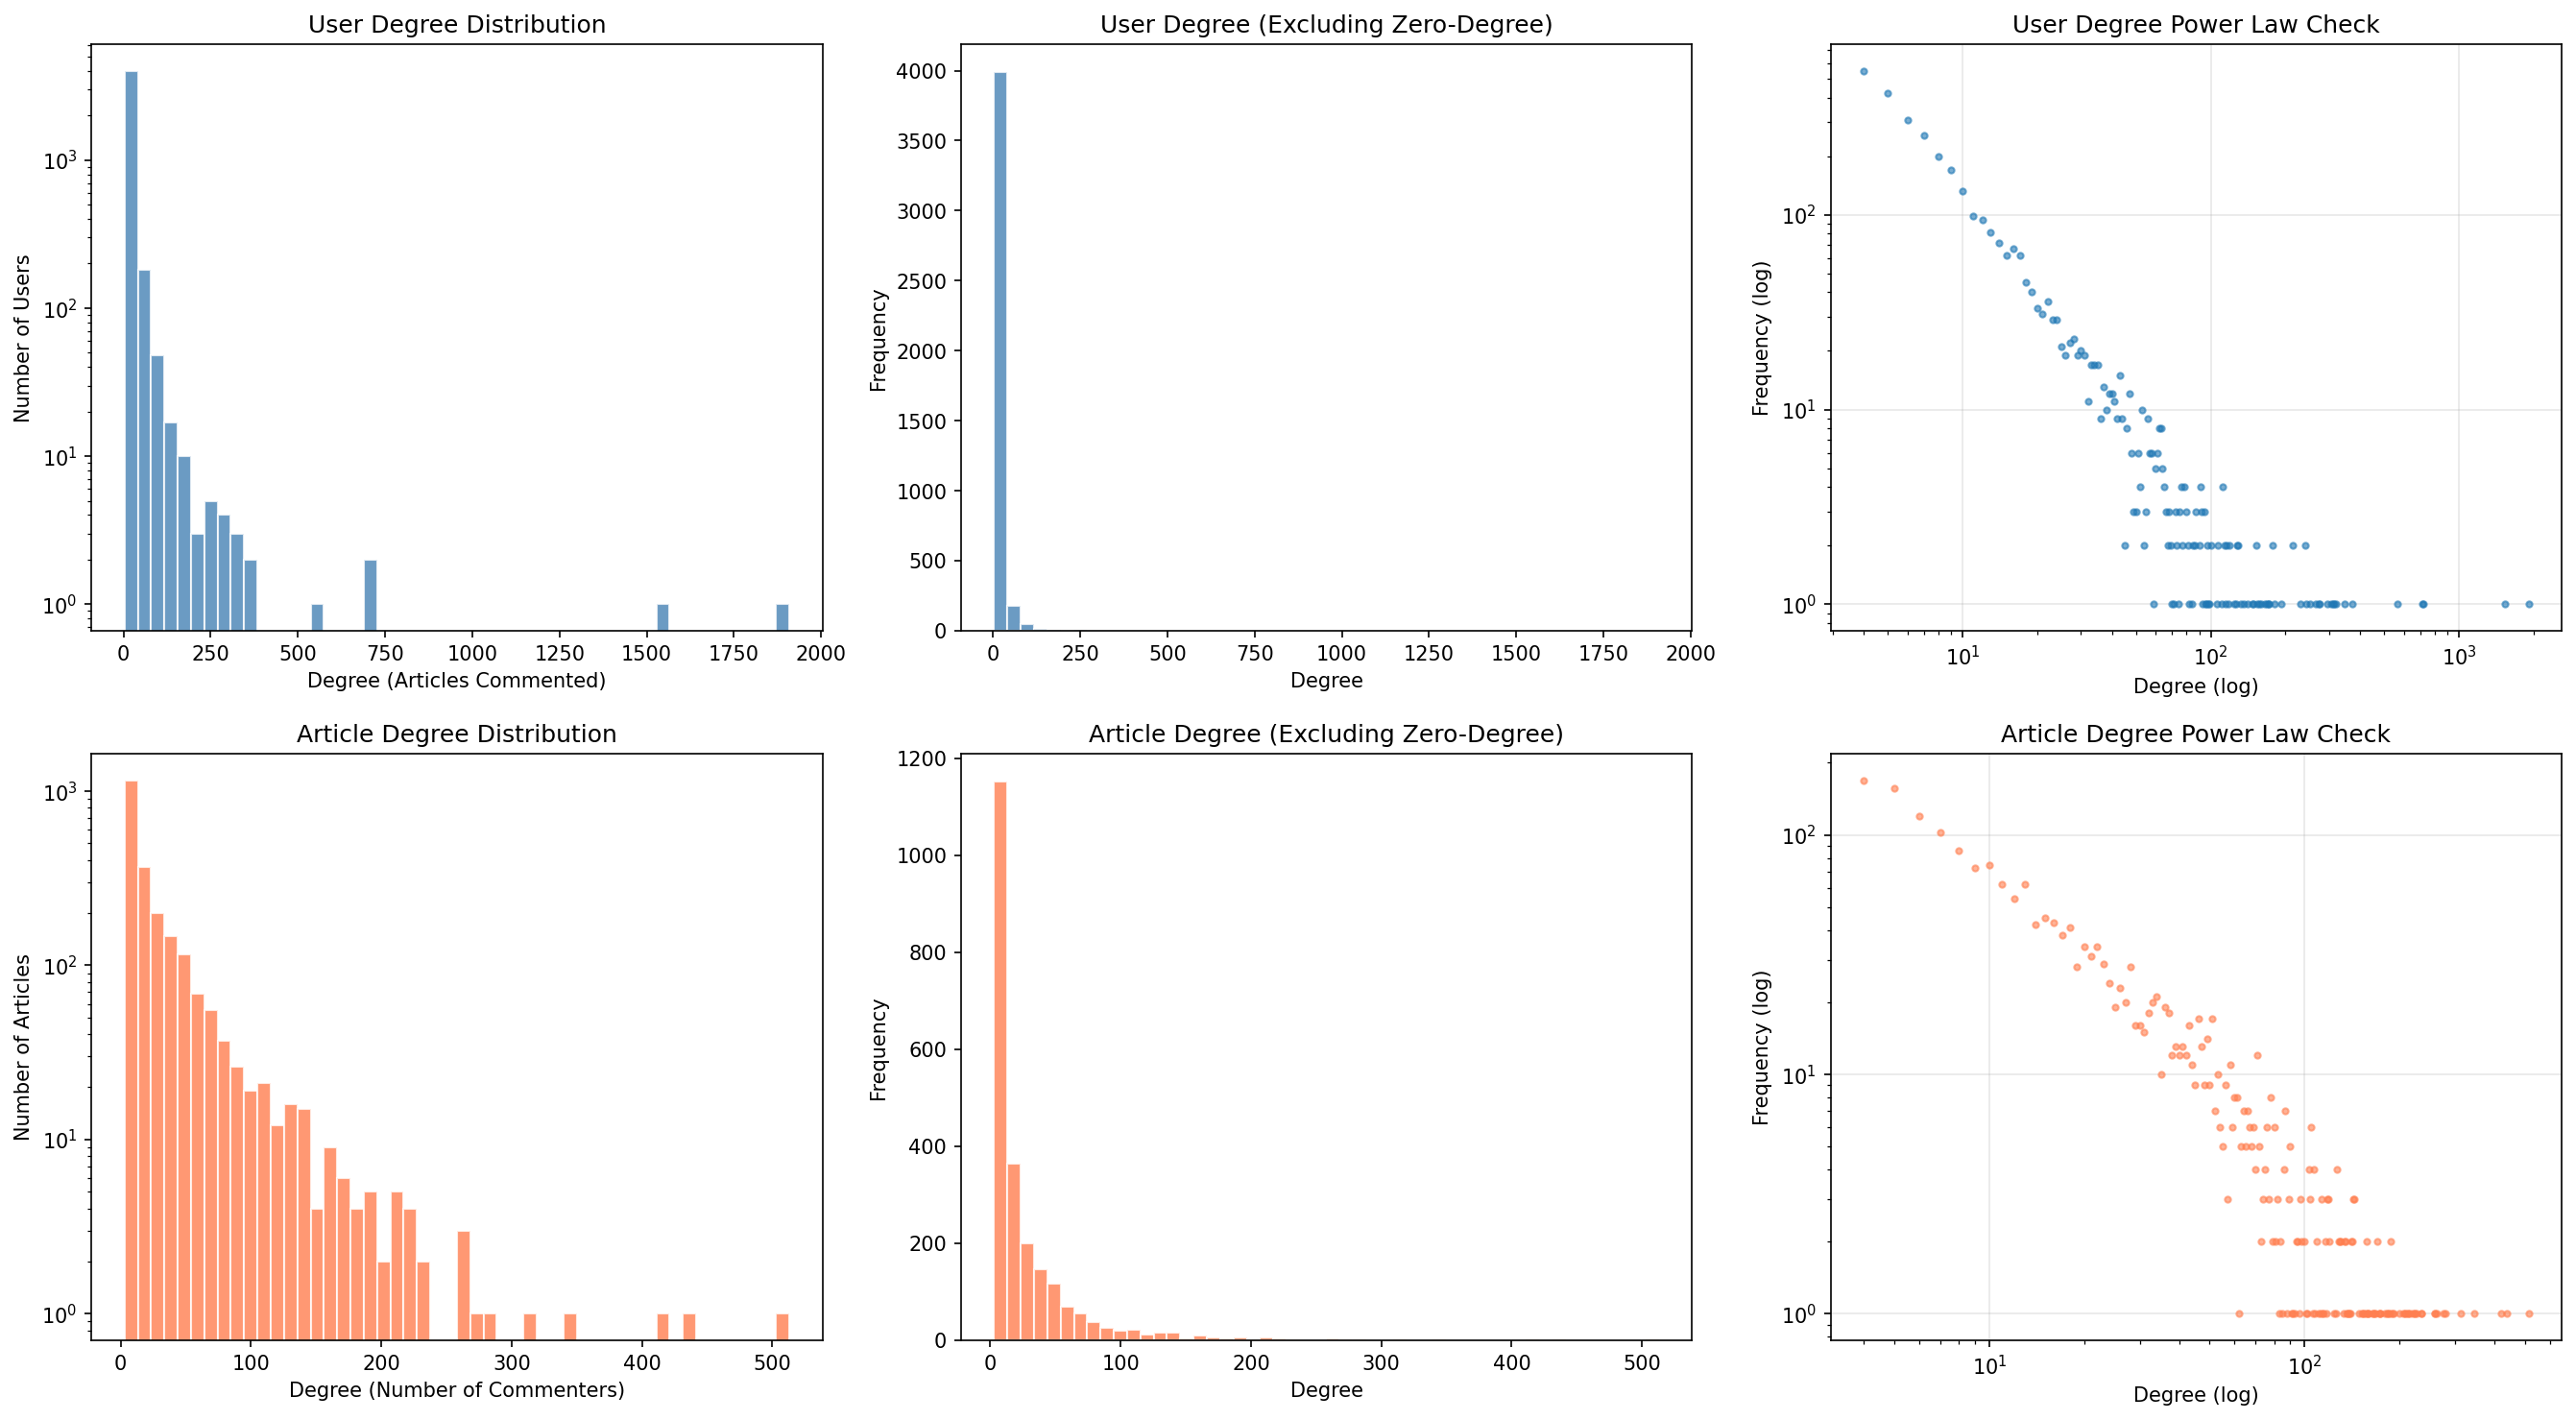
\includegraphics[width=0.9\textwidth]{../plots/graph_eda_01_degree_distribution.png}
% \end{frame}

% \begin{frame}
%     \frametitle{Feature Distribution}
%     \centering
%     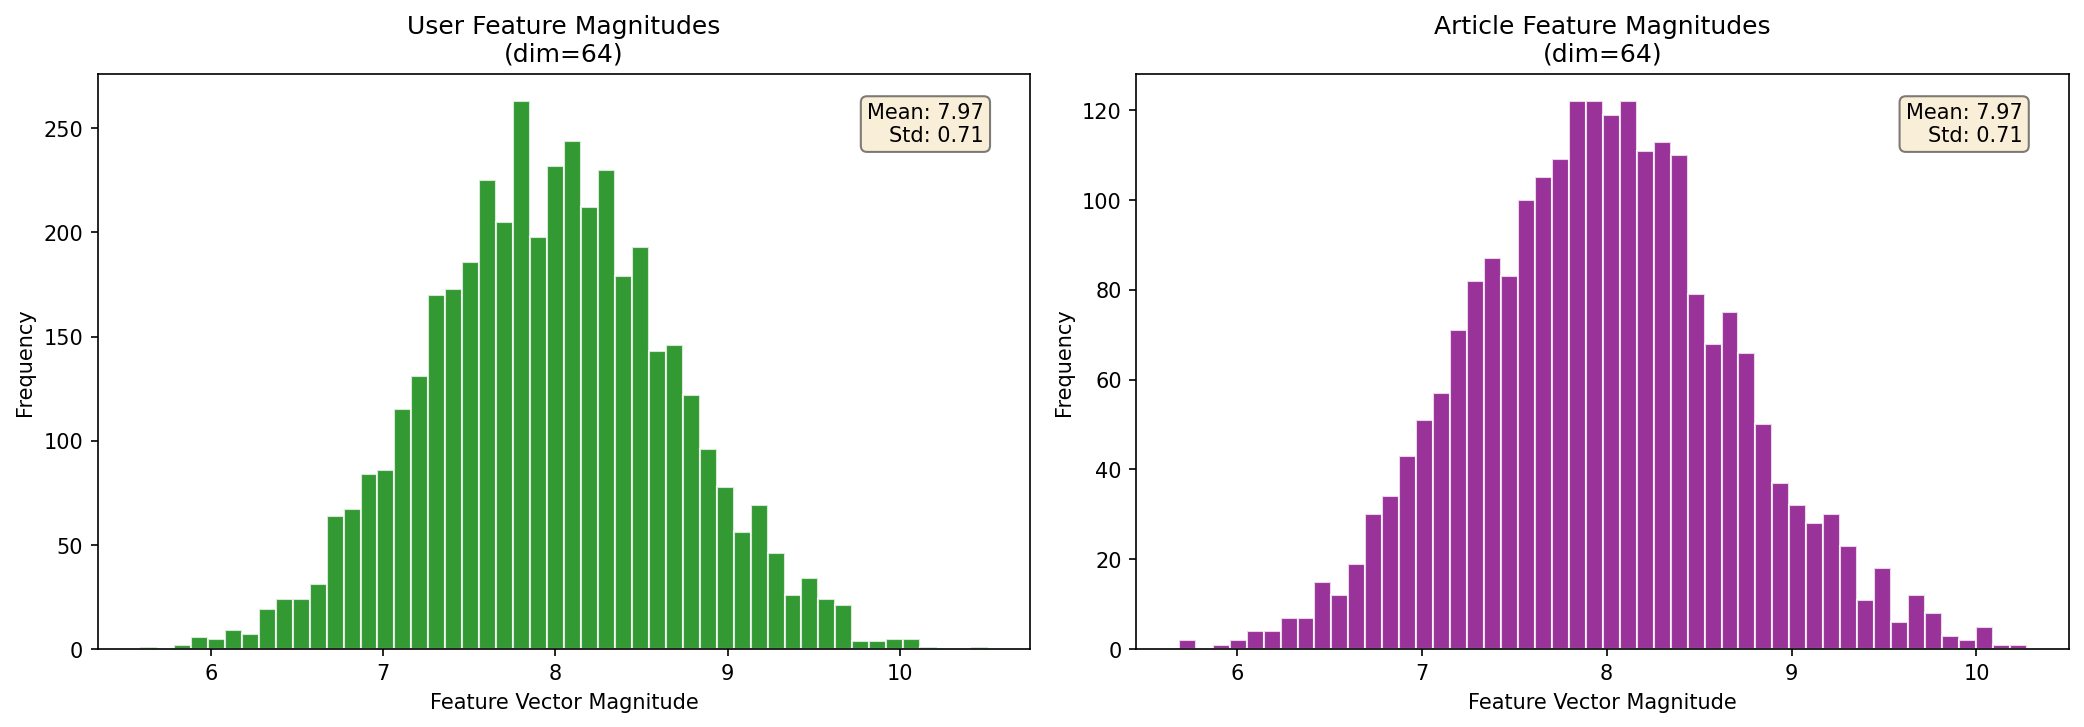
\includegraphics[width=0.9\textwidth]{../plots/graph_eda_02_feature_distribution.png}
% \end{frame}

% \begin{frame}
%     \frametitle{Graph Connectivity}
%     \centering
%     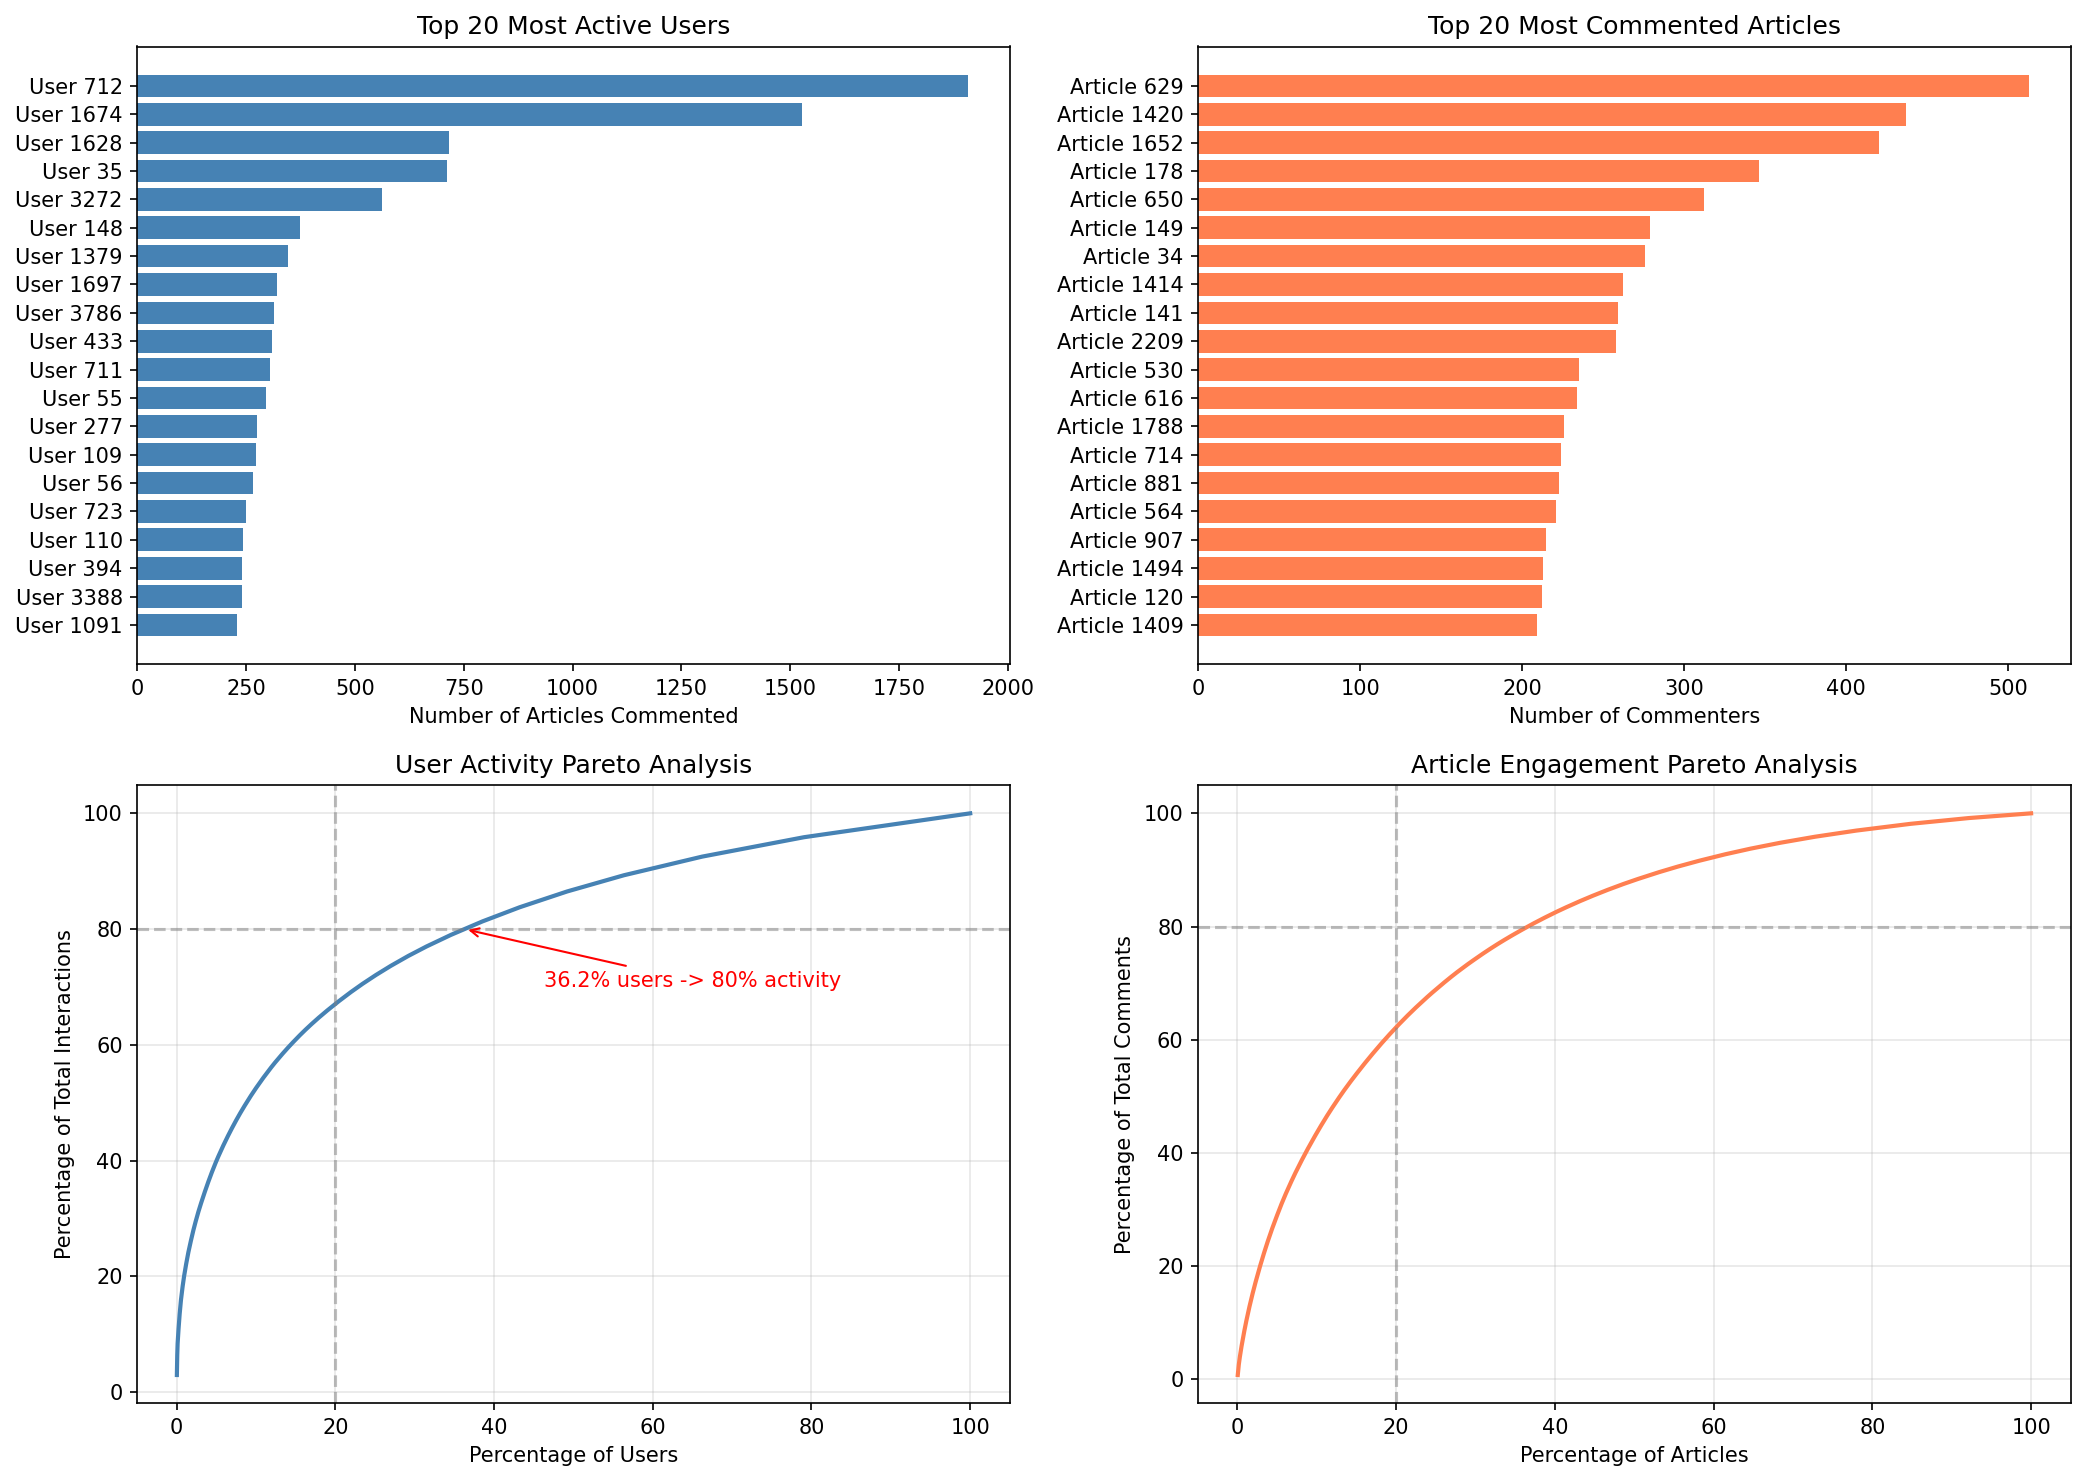
\includegraphics[width=0.9\textwidth]{../plots/graph_eda_03_connectivity.png}
% \end{frame}

%------------------------------------------------------------
\section{Experimental Results}
%------------------------------------------------------------

\begin{frame}
    \frametitle{Model Comparison (PhoBERT, min\_interactions=5)}
    \small
    \begin{table}
        \centering
        \begin{tabular}{l|c|ccc|c}
            \toprule
            \textbf{Model} & \textbf{Type} & \textbf{R@1}   & \textbf{R@5}   & \textbf{R@10}  & \textbf{MRR}   \\
            \midrule
            \textbf{SGL}   & CL            & \textbf{0.802} & \textbf{0.924} & \textbf{0.965} & \textbf{0.879} \\
            NCL            & CL            & 0.811          & 0.890          & 0.917          & 0.868          \\
            SimGCL         & CL            & 0.706          & 0.854          & 0.902          & 0.795          \\
            \midrule
            DirectAU       & CF            & 0.000          & 0.013          & 0.024          & 0.006          \\
            NGCF           & CF            & 0.003          & 0.010          & 0.021          & 0.011          \\
            SimpleX        & CF            & 0.003          & 0.010          & 0.019          & 0.007          \\
            LightGCL       & CL            & 0.013          & 0.010          & 0.016          & 0.016          \\
            \bottomrule
        \end{tabular}
        \caption{Performance on VnExpress dataset (30 epochs)}
    \end{table}
\end{frame}


%------------------------------------------------------------
%------------------------------------------------------------
\begin{frame}
    \centering
    \Huge \textbf{Thank You!}

    \vspace{1cm}
    \large Q \& A
\end{frame}
%------------------------------------------------------------

\end{document}
